\documentclass{article}
\usepackage[utf8]{inputenc}
% \usepackage[english,greek]{babel}
\usepackage[unicode]{hyperref}
\usepackage[LGR, T1]{fontenc}
\usepackage{amsfonts, alphabeta, amssymb}
\usepackage[none]{hyphenat}
\usepackage{amsmath, slashed, graphicx, physics, tikz, braket, caption, subfig, comment, geometry, multicol, lipsum, fancyhdr, tcolorbox, siunitx, authblk, xcolor, abstract, float, indentfirst, xfrac, cancel, bbold, appendix, tikz, tikz-feynman, tensor, multirow, makecell, algpseudocode, algorithmicx, algorithm, changepage, adjustbox, lscape, placeins}
\usepackage[style=numeric-comp,sorting=none]{biblatex}
\addbibresource{references.bib}
\setcounter{secnumdepth}{3}
\setcounter{tocdepth}{3}
\title{\textbf{
        Study of a new kinematic weighting algorithm for the measurement of CP asymmetries in charm decays}
        \\
        LHCb Collaboration
}
\author{
        Georgios Christou
        \\
        Supervisors: Dr.\@ Federico Betti, Prof.\@ Angelo Carbone
}
\date{
        August 2023
}

\begin{document}
        \begin{figure}[t]
                \centering
                \subfloat{
\includegraphics[height = 3.5cm]{../.images/CERN_logo.png}}
                \hspace{1cm}
                \subfloat{
\includegraphics[height = 3.5cm]{../.images/Lhcb-logo-new.svg.png}}
        \end{figure}

        \maketitle

        \begin{abstract}
                We investigate the asymmetries that occur in charm decays at the LHCb, specifically we study $D^{\star+}\to D^0\pi^+$ and $\bar{D}^{\star-}\to D^0\pi^-$ where $D^0\to K^-K^+$ or $D^0\to \pi^-\pi^+$.
                We study the effect of $CP$ and detection asymmetries on MC samples generated via RapidSim and implement a new kinematic weighting function which allows us to keep events that are otherwise discarded from LHCb data, since they are associated with large detection asymmetries.
        \end{abstract}
        
        \pagebreak
        % \tableofcontents
        % \pagebreak

        \section{Introduction}
        We investigate charm decays and specifically the $D^\star$ meson.
        By studying the differences between $D^{\star +}$ and $D^{\star -}$ decays shown in Fig. \ref{fig:diagrams} we can estimate the $CP$ asymmetry in charm decays.
        \begin{figure}[h!]
                \centering
                \subfloat{
                        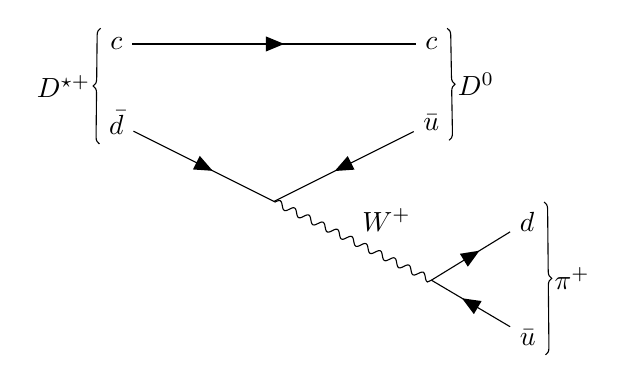
\begin{tikzpicture}
                                \begin{feynman}
                                        \vertex (DStarC) {$c$};
                                        \vertex[below = 1cm of DStarC] (DStarDBar) {$\bar{d}$};

                                        \vertex[right = 4cm of DStarC] (D0C) {$c$};
                                        \vertex[right = 4cm of DStarDBar] (D0UBar) {$\bar{u}$};

                                        \vertex[below right = 1cm and 2cm of DStarDBar] (WStart);
                                        \vertex[below right = 1cm and 2cm of WStart] (WEnd);

                                        \vertex[above right = 0.5cm and 1cm of WEnd] (PiD) {$d$};
                                        \vertex[below right = 0.5cm and 1cm of WEnd] (PiUBar) {$\bar{u}$};
                                        \diagram*{
                                                (DStarC) -- [fermion] (D0C);
                                                (DStarDBar) -- [fermion] (WStart);
                                                (D0UBar) -- [fermion] (WStart);
                                                (WStart) -- [photon, edge label = $W^+$] (WEnd);
                                                (PiUBar) -- [fermion] (WEnd);
                                                (WEnd) -- [fermion] (PiD);
                                        };
                                        \draw [decoration={brace}, decorate] (DStarDBar.south west) -- (DStarC.north west) node [pos=0.5, left] {$D^{\star +}$};
                                        \draw [decoration={brace}, decorate] (D0C.north east) --  (D0UBar.south east) node [pos=0.5, right] {$D^0$};
                                        \draw [decoration={brace}, decorate] (PiD.north east) --  (PiUBar.south east) node [pos=0.5, right] {$\pi^+$};
                                \end{feynman}
                        \end{tikzpicture}
                }
                \subfloat{
                        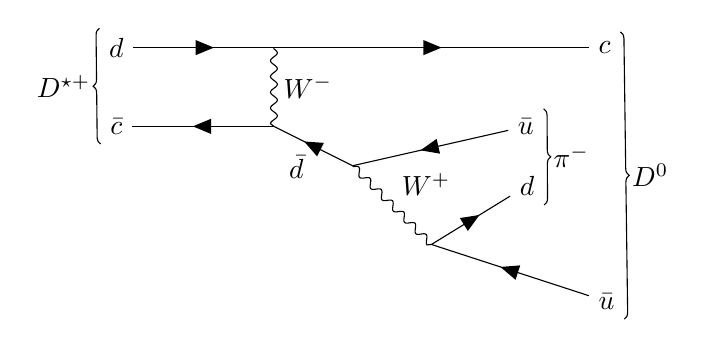
\begin{tikzpicture}
                                \begin{feynman}
                                        \vertex (DStarD) {$d$};
                                        \vertex[below = 1cm of DStarD] (DStarCBar) {$\bar{c}$};

                                        \vertex[right = 6.2cm of DStarD] (D0C) {$c$};
                                        \vertex[right = 5.2cm of DStarCBar] (D0UBar) {$\bar{u}$};

                                        \vertex[right = 2cm of DStarD] (WMinusStart);
                                        \vertex[right = 2cm of DStarCBar] (WMinusEnd);

                                        \vertex[below right = 0.5cm and 1cm of WMinusEnd] (mid);

                                        \vertex[below right = 1cm and 1cm of mid] (W);

                                        \vertex[above right = 0.5cm and 1cm of W] (PiD) {$d$};
                                        \vertex[below right = 0.5cm and 2cm of W] (PiUBar) {$\bar{u}$};

                                        \diagram*{
                                                (DStarD) --[fermion] (WMinusStart);
                                                (WMinusStart) --[fermion] (D0C);
                                                (WMinusStart) --[photon, edge label = $W^-$] (WMinusEnd);
                                                (D0UBar) --[fermion] (mid);
                                                (mid) --[fermion, edge label = $\bar{d}$] (WMinusEnd);
                                                (WMinusEnd) --[fermion] (DStarCBar);
                                                (mid) --[photon, edge label = $W^+$] (W);
                                                (PiUBar) -- [fermion] (W);
                                                (W) -- [fermion] (PiD);
                                        };
                                        \draw [decoration={brace}, decorate] (DStarCBar.south west) -- (DStarD.north west) node [pos=0.5, left] {$D^{\star +}$};
                                        \draw [decoration={brace}, decorate] (D0C.north east) --  (PiUBar.south east) node [pos=0.5, right] {$D^0$};
                                        \draw [decoration={brace}, decorate] (D0UBar.north east) --  (PiD.south east) node [pos=0.5, right] {$\pi^-$};
                                \end{feynman}
                        \end{tikzpicture}
                }
                \caption{Feynman diagram showing $D^{\star \pm}\to D^{0} \pi^{\pm}$ decays.}
                \label{fig:diagrams}
        \end{figure}

        The total asymmetry one observes at an experiment is a combination of multiple asymmetries.
        Namely, the total asymmetry consists of a \textit{CP asymmetry} and a \textit{detection asymmetry}.
        The former is associated with the difference between matter and anti-matter, while the latter is associated with the differences while detecting the soft pion $(\pi_s)$ that is produced during the decay.

        The total asymmetry can be estimated using 
        \begin{equation}
                \label{eq:total}
                A_\text{total} = \frac{A_{CP} + A_\text{D}}{1 + A_{C}A_\text{D}}
        \end{equation}
        where $A_{CP}$ and $A_\text{D}$ are the $CP$ and \textit{integrated detection asymmetries}.
        The latter can be calculated through
        \begin{equation}
                A_\text{D} = \frac{\int \dd \vec{p} N(\vec{p})A_\text{D}(\vec{p})}{\int \dd \vec{p} N(\vec{p})}
        \end{equation}


        At the LHCb one observes large pion detection asymmetries that are associated with specific kinematic regions, which so far have been discarded, thus reducing the statistics.
        We can, however, introduce a \textit{weighting function} that allows us to keep events in these kinematic regions.
        Such a weighting function can be expressed as the following ratio
        \begin{equation}
                \label{eq:weighting}
                Q(\vec{p}_{D^\star}, \vec{p}_{\pi_s}) \simeq \frac{\Gamma_{D^0}^{\pi\pi}(\vec{p}_{D^\star} - \vec{p}_{\pi_s}) + \Gamma_{\bar{D}^0}^{\pi\pi}(\vec{p}_{D^\star} - \vec{p}_{\pi_s})}{\Gamma_{D^0}^{KK}(\vec{p}_{D^\star} - \vec{p}_{\pi_s}) + \Gamma_{\bar{D}^0}^{KK}(\vec{p}_{D^\star} - \vec{p}_{\pi_s})}
        \end{equation}
        where $\Gamma_{D^{0}/\bar{D}^0}^{\pi\pi/KK}$ are the normalized distributions of $D^0$ candidates.
        Unfortunately in Run-2 such candidates were discarded, thus, we do not have a large enough sample to accurately calculate the weighting function and we resort to Monte Carlo simulations.

        
        \section{Analysis}
        \subsection{RapidSim}
        For the analysis we make use of the RapidSim simulation \cite{Cowan:2016tnm} to generate $D^{\star \pm}\to D^0 \pi^\pm$ events where $D^0$ subsequently decays into $K^-K^+$ or $\pi^-\pi^+$.
        We present the RapiDSim parameters in Tab. \ref{tab:RapidSim}

        \begin{center}
                \begin{tabular}{c|c|c}
                        & Parameter & Value\\
                        \hline\hline
                        Center of mass energy & \texttt{energy} &               \texttt{13}\\
                        Detector geometry & \texttt{geometry} &                 \texttt{LHCb}\\
                        Acceptance region & \texttt{acceptance} &               \texttt{AllIn}\\
                        Smearing on produced particles & \texttt{smear} &       \texttt{LHCbGeneric}
                \end{tabular}
                \captionof{table}{RapidSim parameters used to generate our data.}
                \label{tab:RapidSim}
        \end{center}

        \subsection{Calculation of the $Q$ function}
        As previously discussed, the weighting function Eq. \ref{eq:weighting} allows us to keep more events from LHCb to more accurate results, thus, the calculation of 
        the weighting function needs to be done correctly and with enough precision.

        We generate separate samples for calculating the weighting function $Q$ and analyzing our data to eliminate correlations between the two.
        Both samples start with 10 million events, to have high enough statistics and then events are discarded due to the selections we applied in Tab. \ref{tab:RapidSim}.

        We calculate the weighting function twice, once with detection asymmetry and once without, and compare the results.
        The detection asymmetry is shown in Fig.~\ref{fig:detection}.
        \begin{figure}[h!]
                \centering
                \subfloat{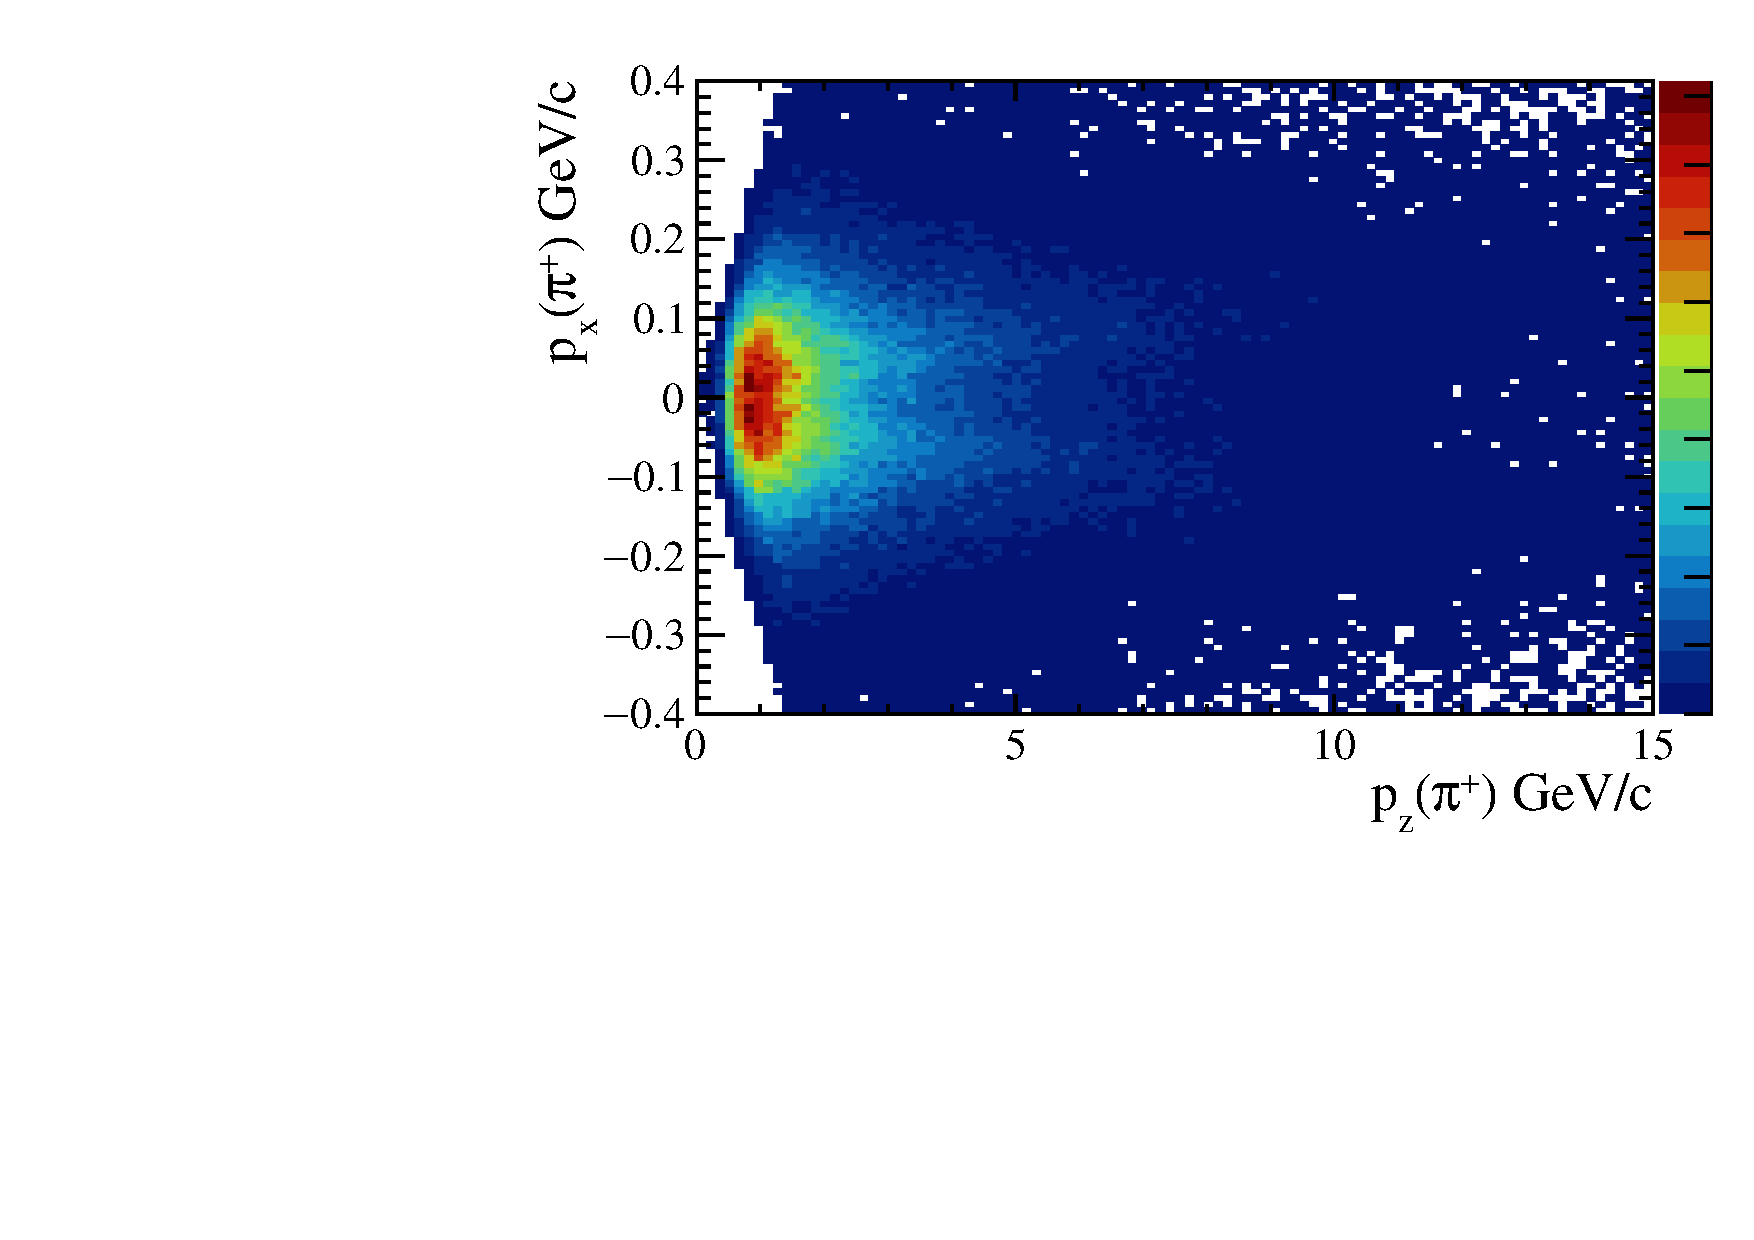
\includegraphics[width = 0.5\textwidth]{../work/RapidSimAnalysis/MomentumDependence/Plots/KK_Dst_PXPZ_Positive.pdf}}
                \subfloat{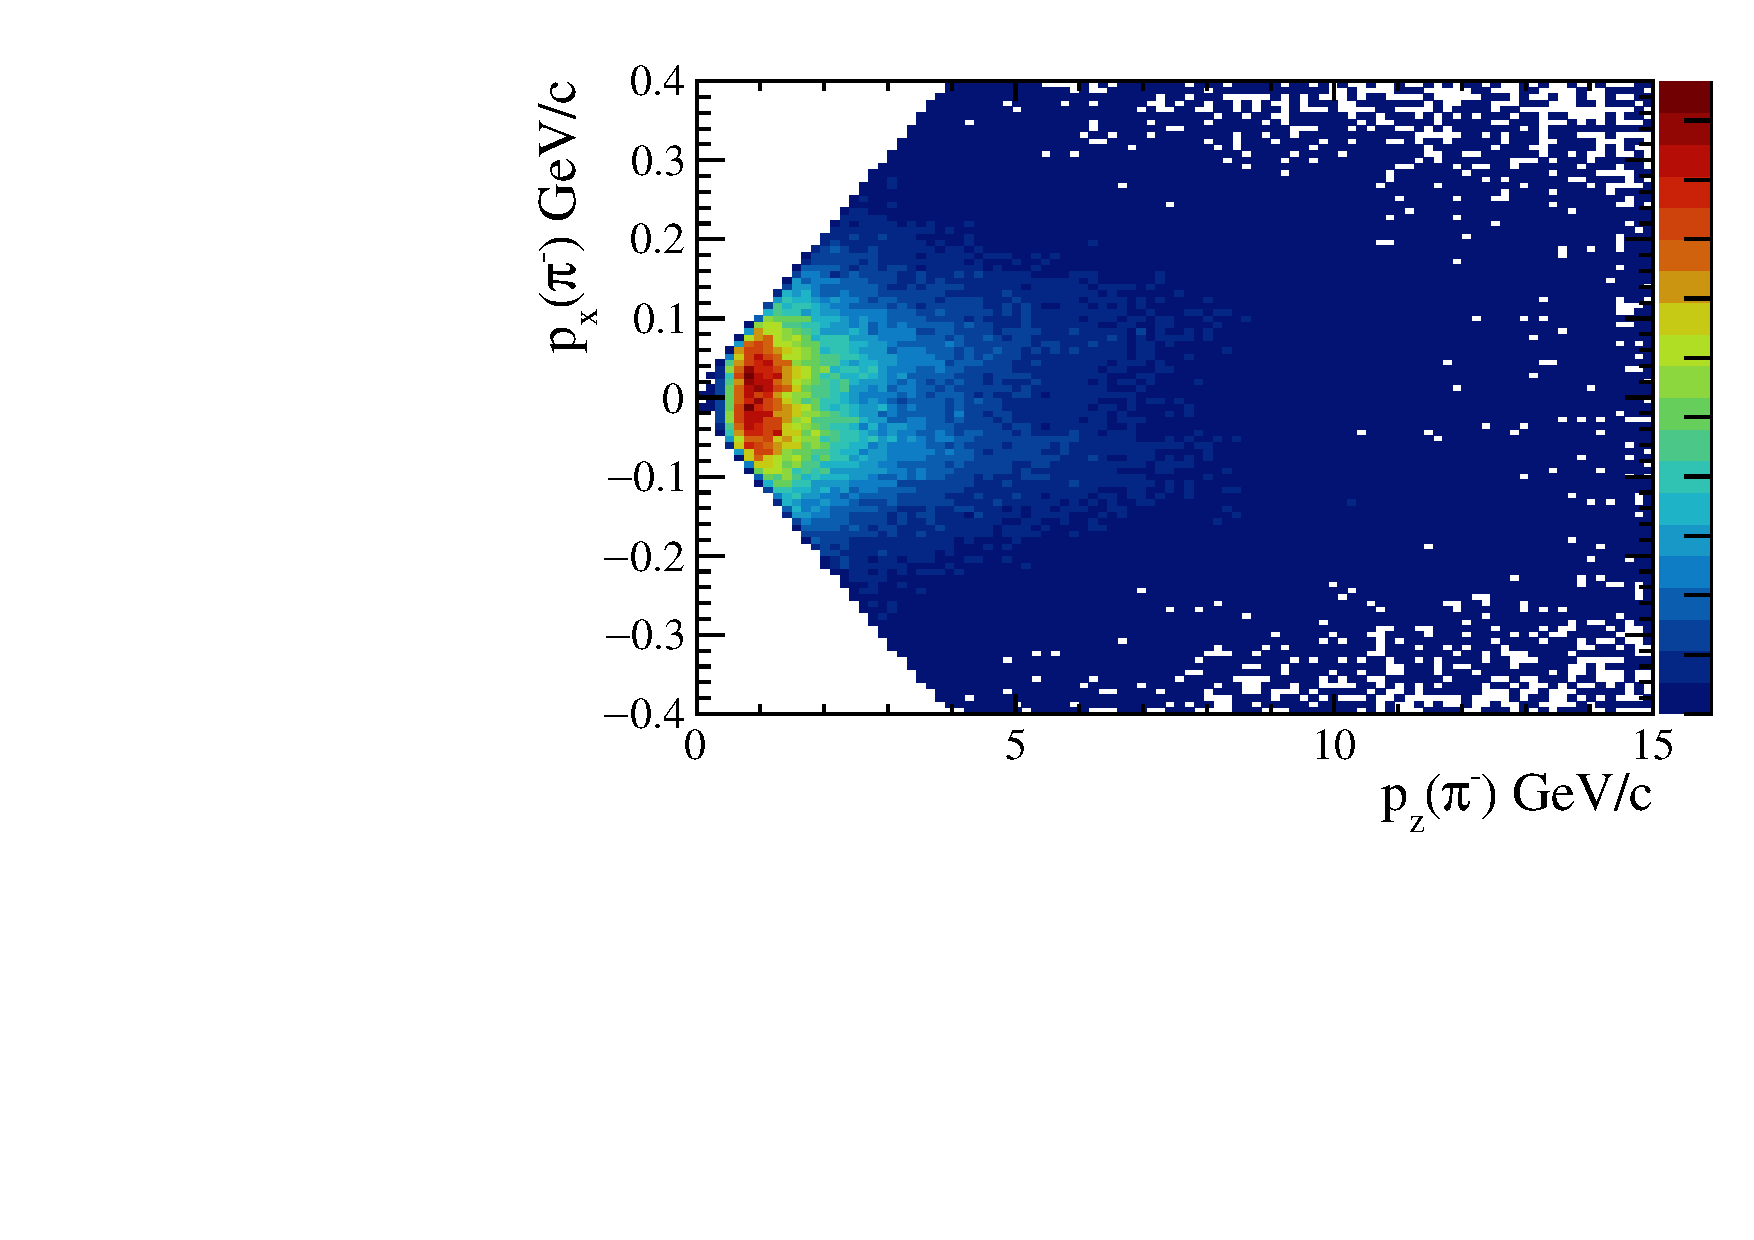
\includegraphics[width = 0.5\textwidth]{../work/RapidSimAnalysis/MomentumDependence/Plots/KK_Dst_PXPZ_Negative.pdf}}
                \caption{Positive and negative soft pion $p_x - p_z$ momentum plane for the $D^0\to k^-K^+$ sample. We add a detection asymmetry only on the negative soft pion.}
                \label{fig:detection}
        \end{figure}

        We present the weighting function distributions for before and after the detection asymmetry in Fig.~\ref{fig:weightsBeforeAfter}.
        \begin{figure}[h!]
                \centering
                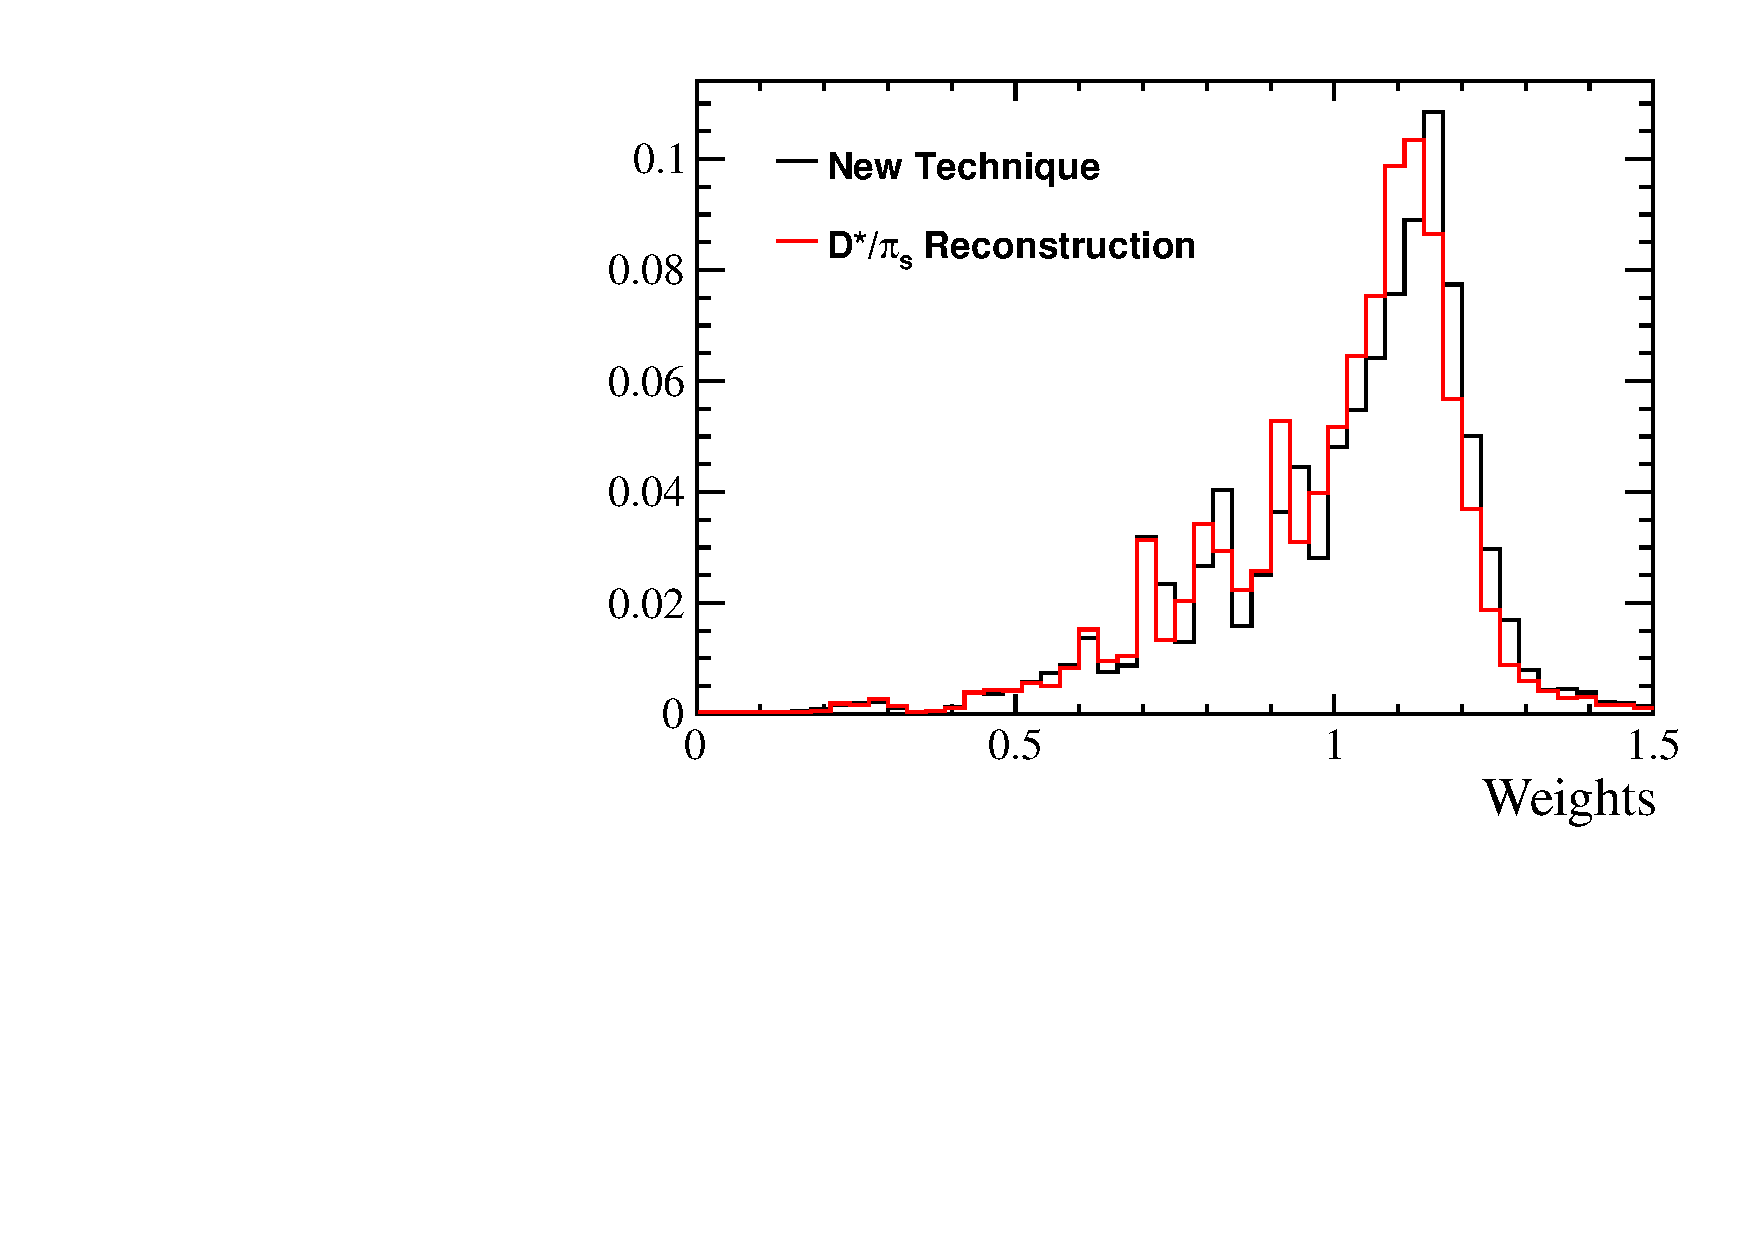
\includegraphics[width = 0.7\textwidth]{../work/RapidSimAnalysis/NewWeightingFunction/Plots/WeighsBeforeAfter.pdf}
                \caption{Distribution of weighting function values before and after the detection asymmetry.}
                \label{fig:weightsBeforeAfter}
        \end{figure}
        It is obvious that the introduction of the detection asymmetry slightly affects the weighting function distribution.
        \begin{figure}[h!]
                \centering
                \subfloat{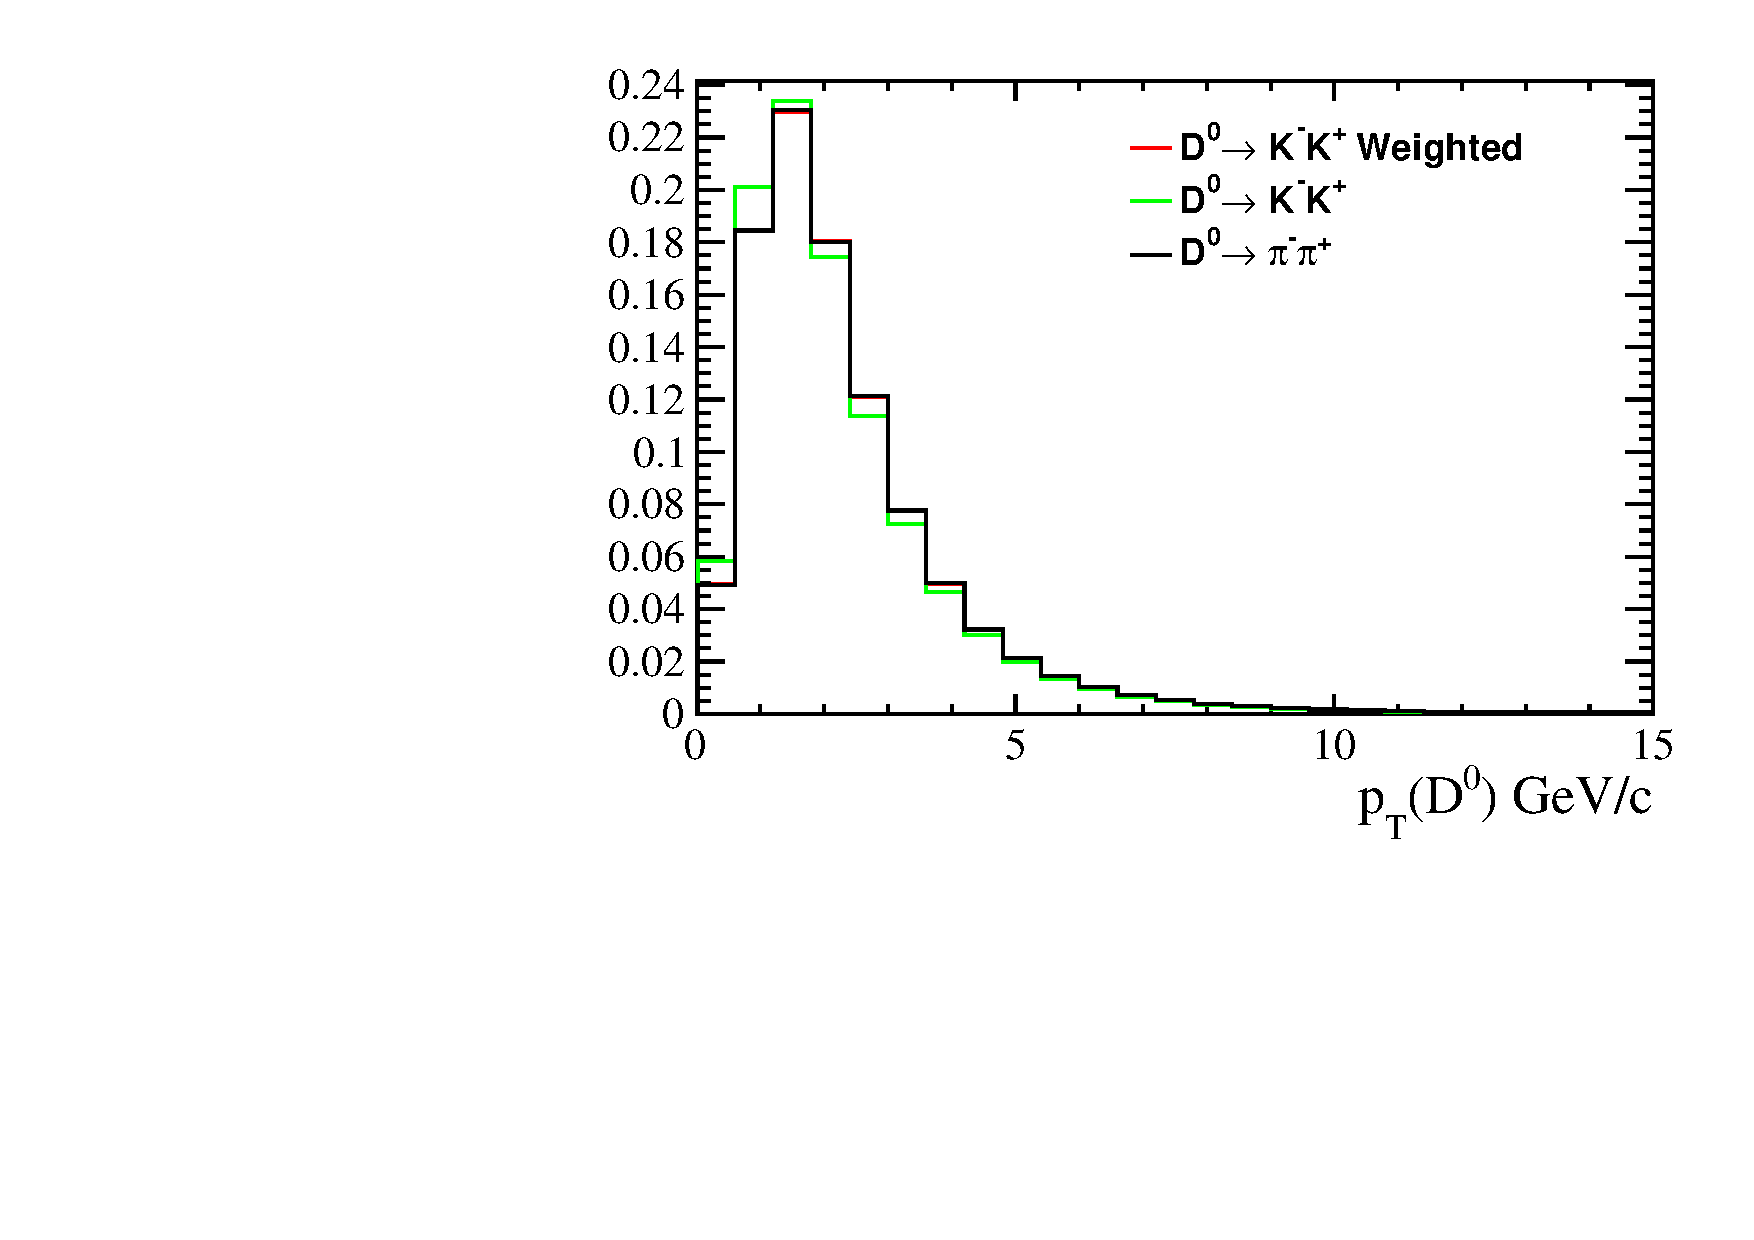
\includegraphics[width = 0.5\textwidth]{../work/RapidSimAnalysis/NewWeightingFunction/Plots/D0_PT_All.pdf}}
                \subfloat{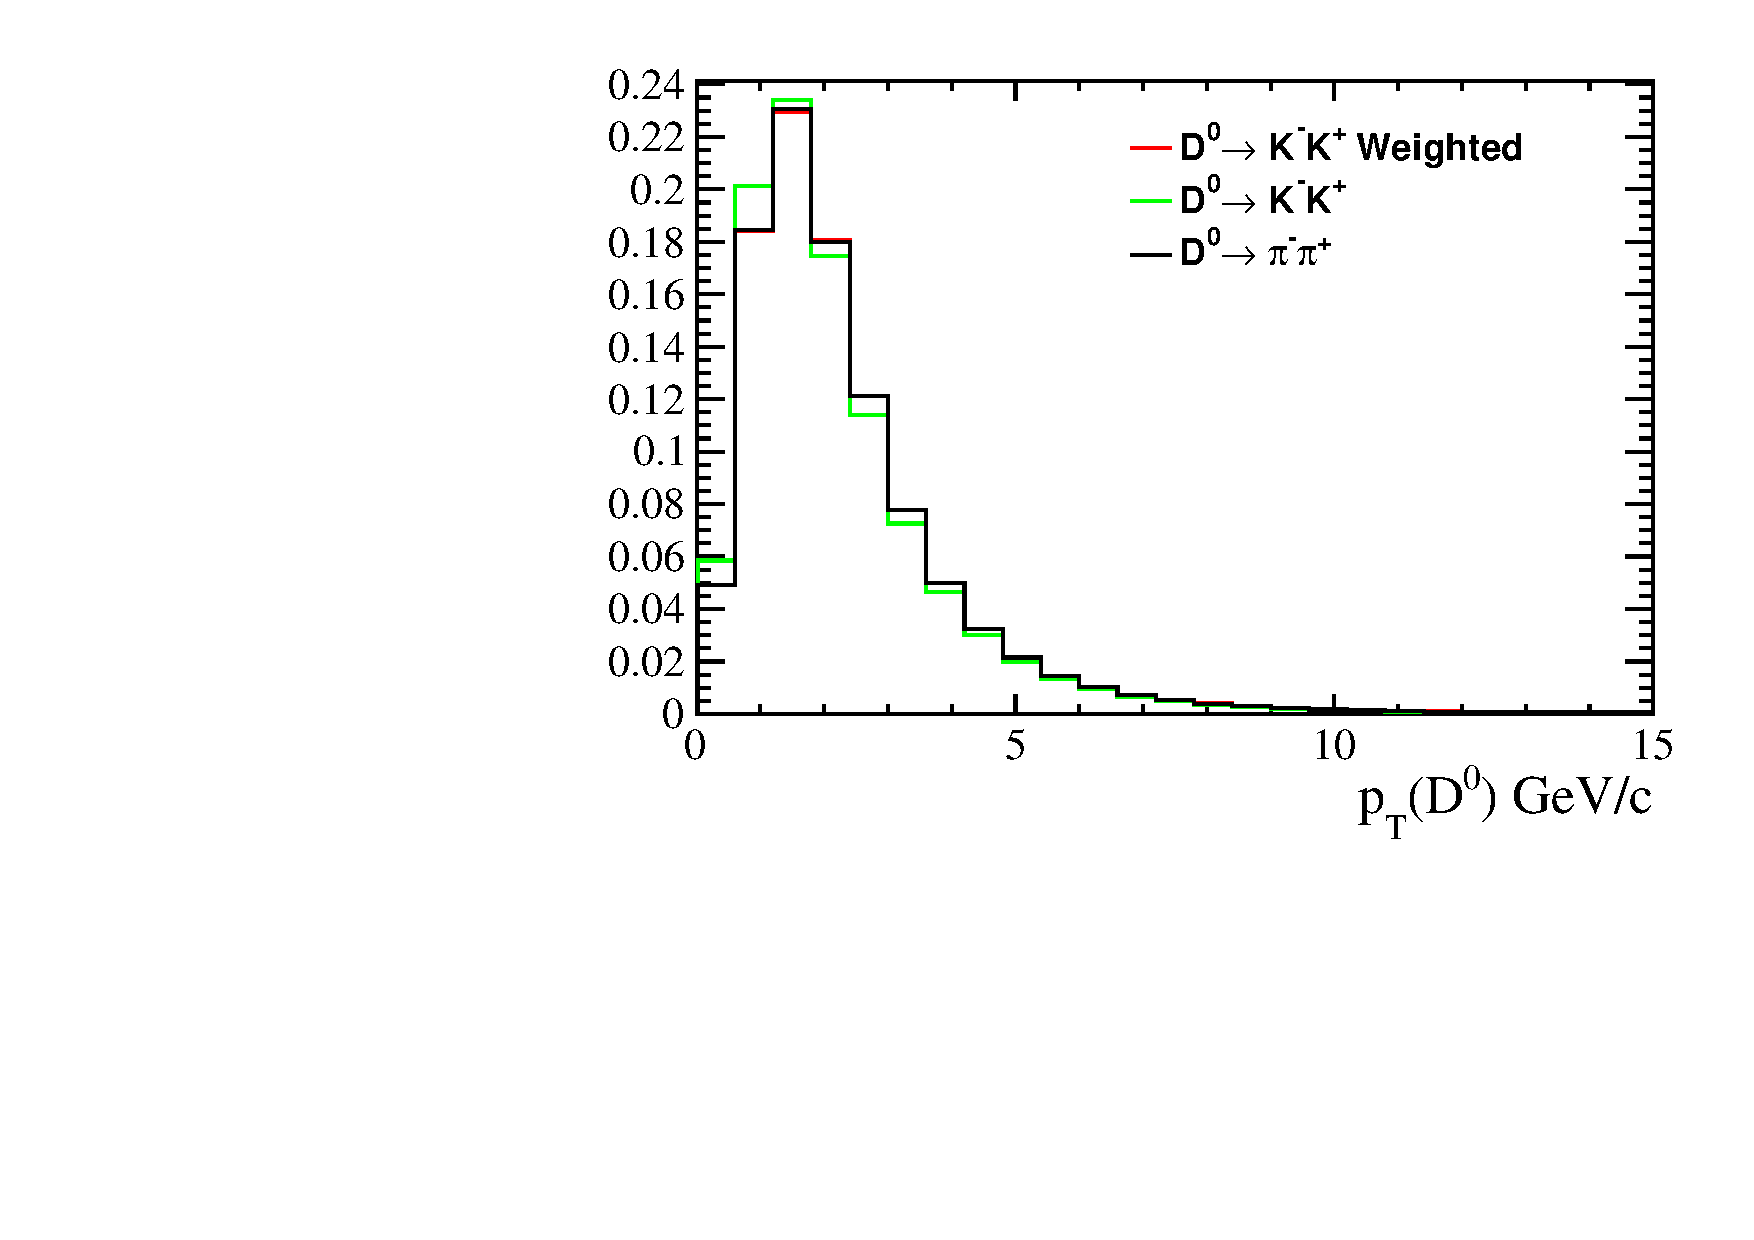
\includegraphics[width = 0.5\textwidth]{../work/RapidSimAnalysis/WeightingFunction/Plots/D0_PT_All.pdf}}

                \hfill

                \subfloat{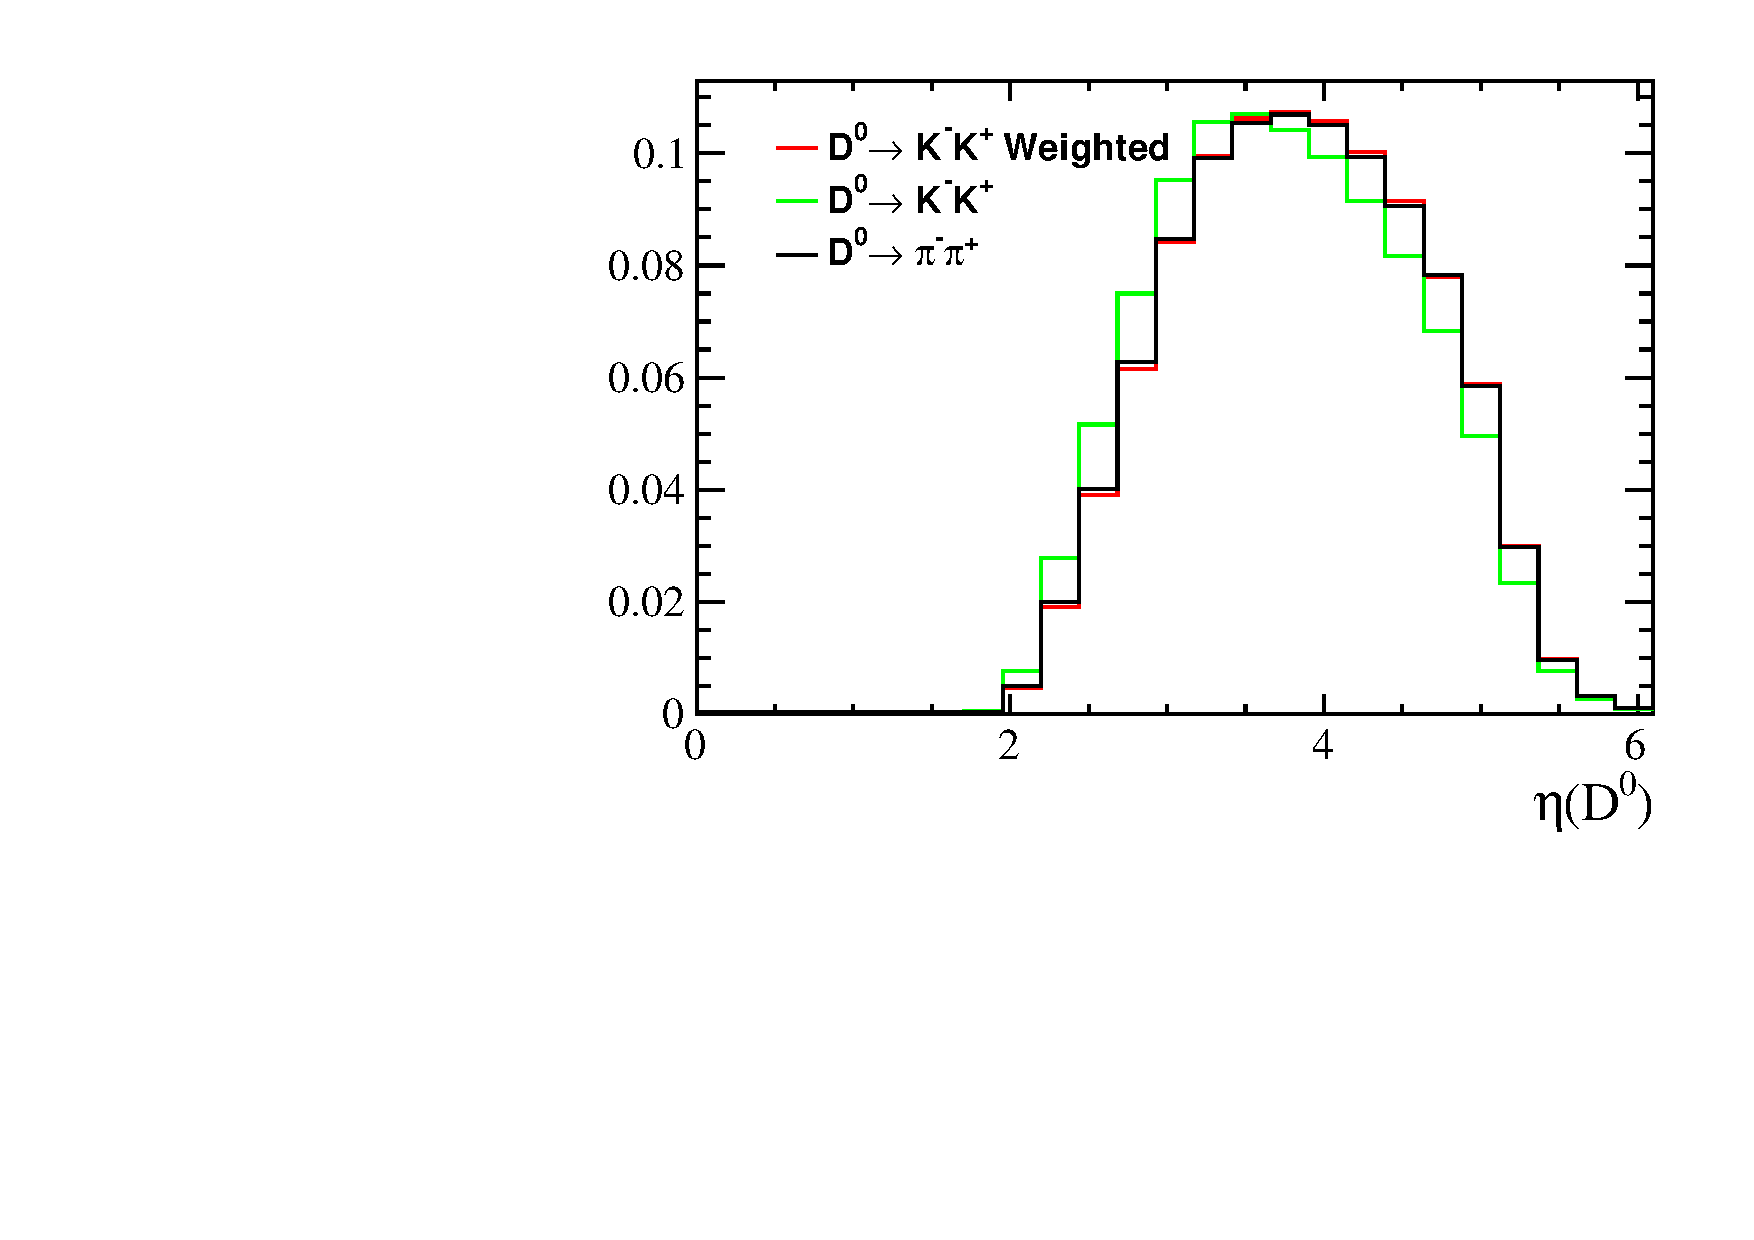
\includegraphics[width = 0.5\textwidth]{../work/RapidSimAnalysis/NewWeightingFunction/Plots/D0_eta_All.pdf}}
                \subfloat{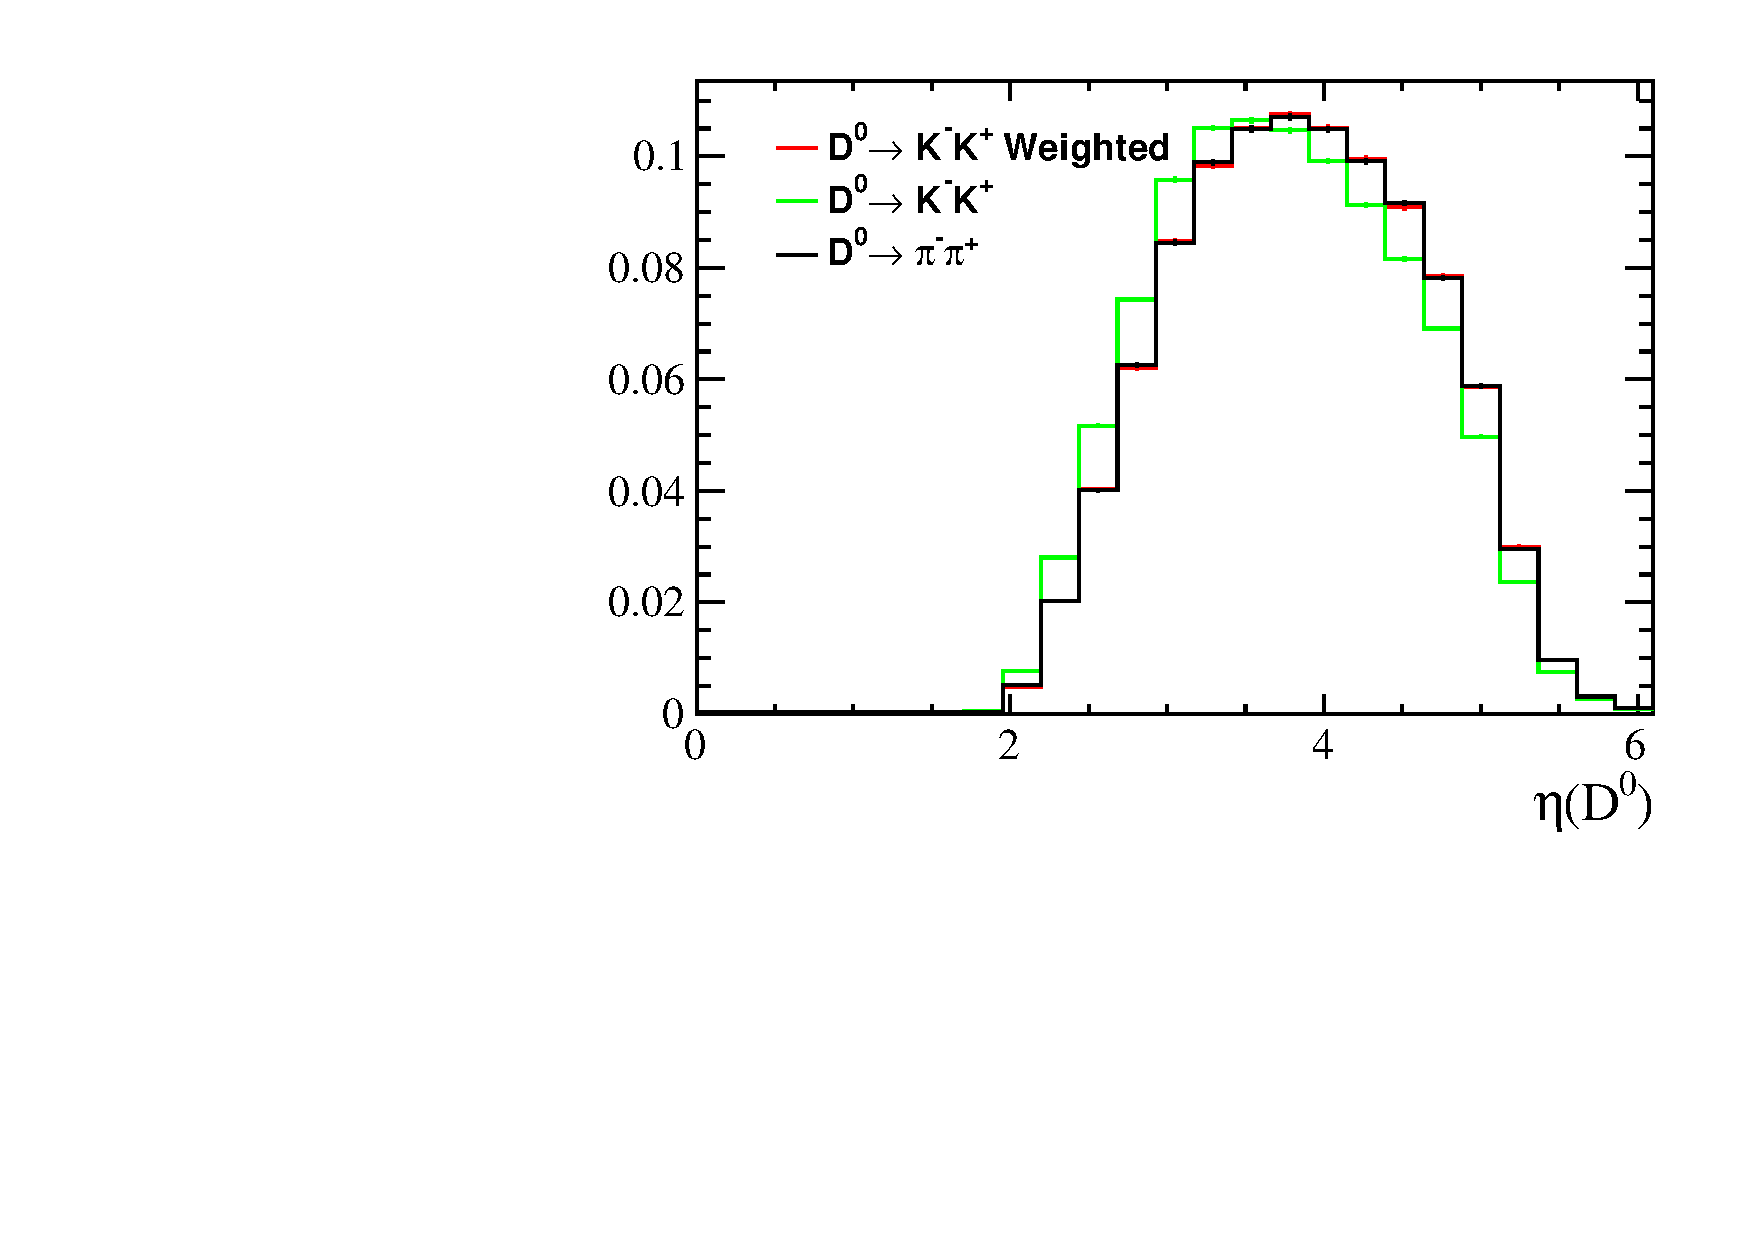
\includegraphics[width = 0.5\textwidth]{../work/RapidSimAnalysis/WeightingFunction/Plots/D0_eta_All.pdf}}

                \hfill

                \subfloat{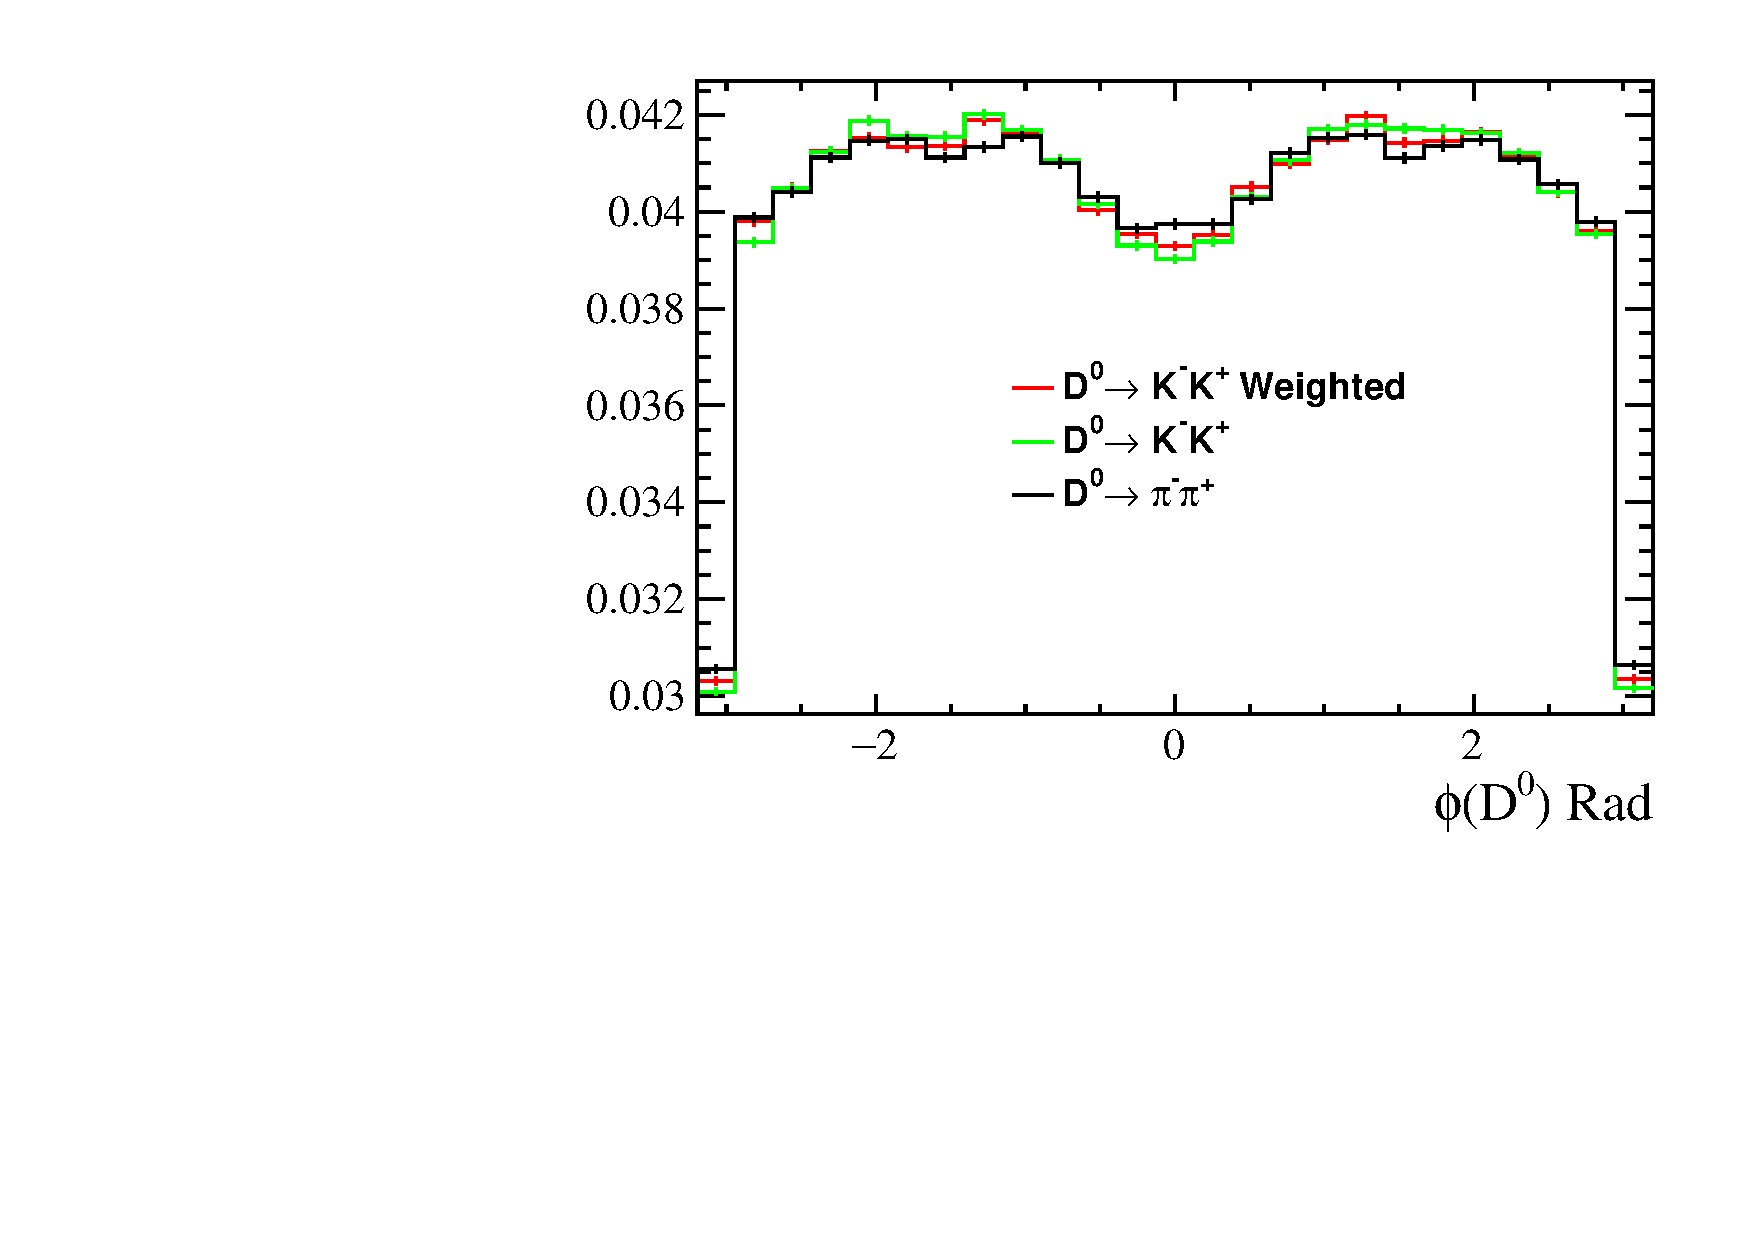
\includegraphics[width = 0.5\textwidth]{../work/RapidSimAnalysis/NewWeightingFunction/Plots/D0_phi_All.pdf}}
                \subfloat{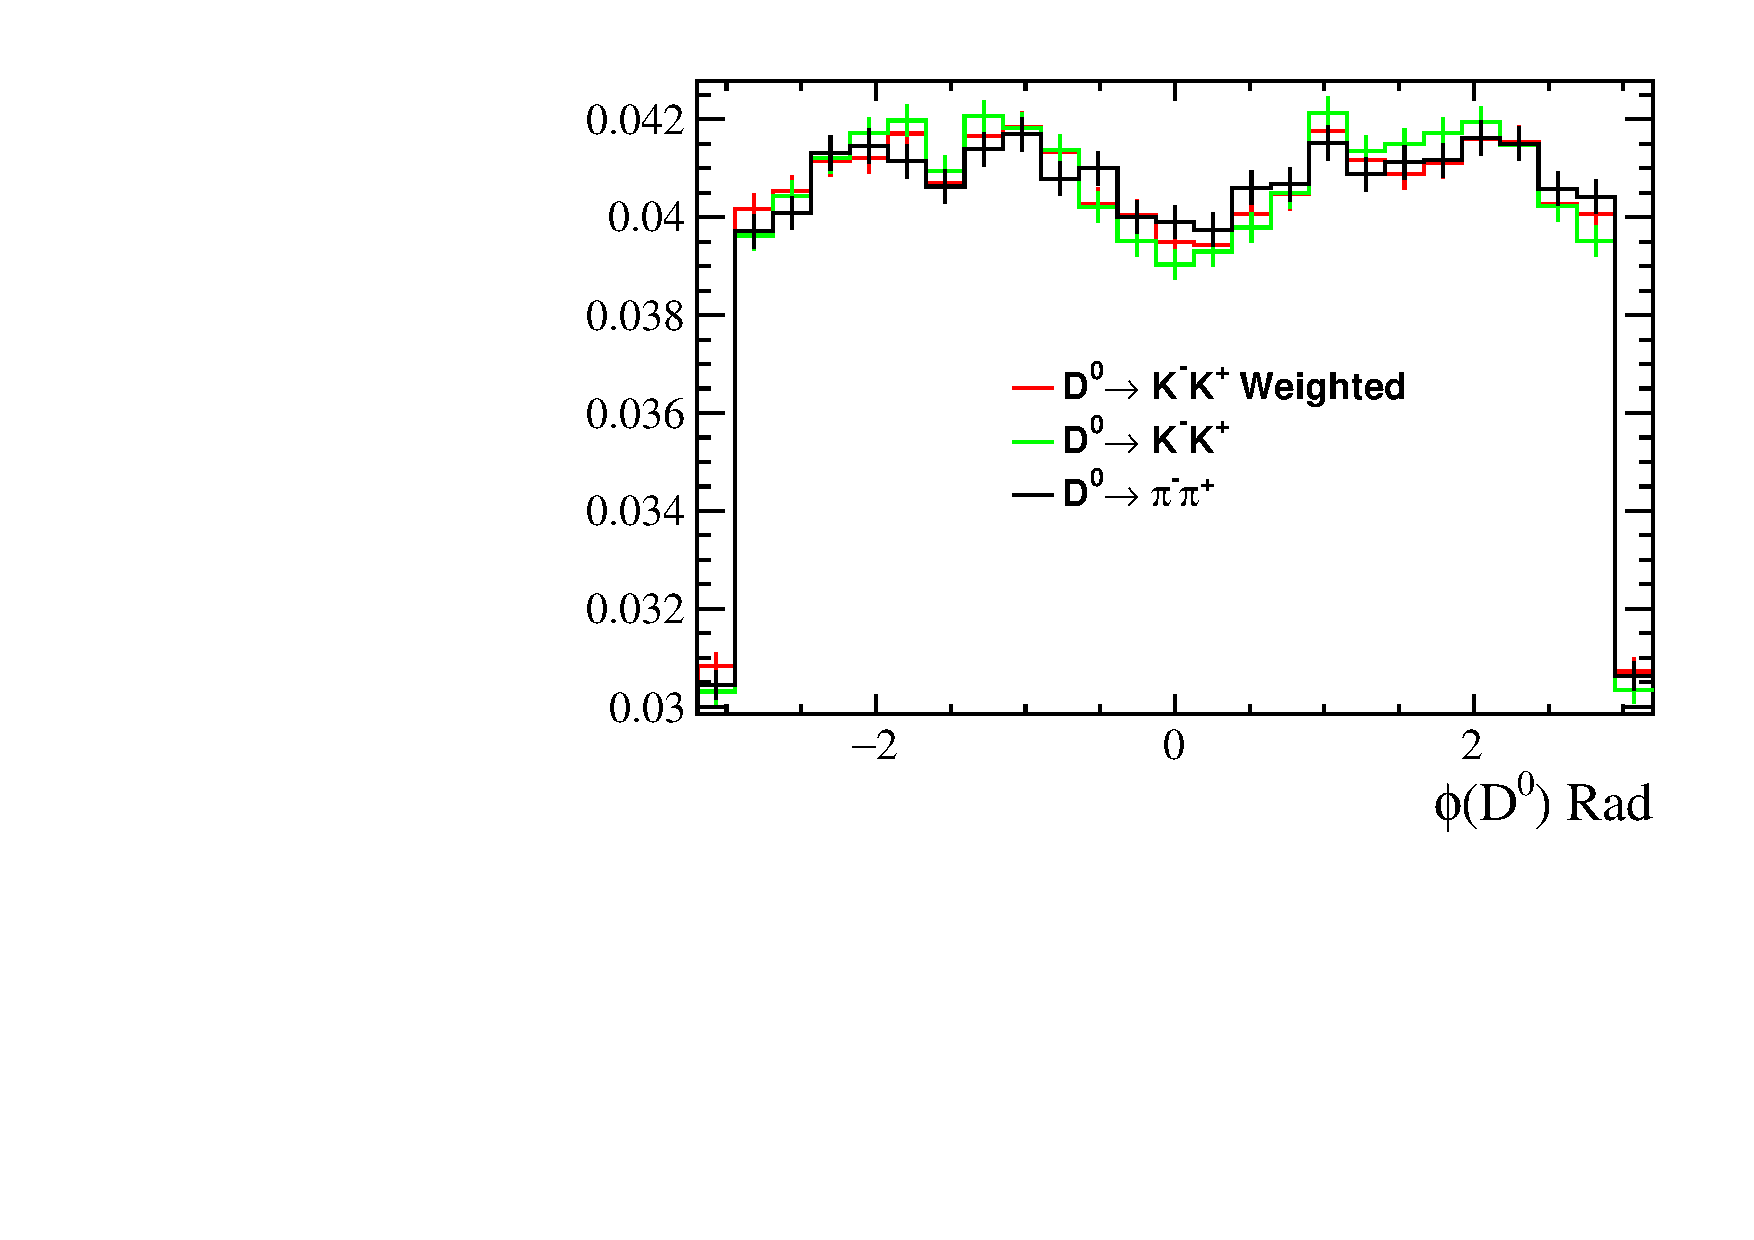
\includegraphics[width = 0.5\textwidth]{../work/RapidSimAnalysis/WeightingFunction/Plots/D0_phi_All.pdf}}

                \caption{Comparison of $D^0$ kinematics with and without weighting. On the left and right columns we present the weighting before and after the introduction of the detection asymmetry respectively.}
        \end{figure}

        \subsection{Asymmetry calculation}
        Using the weighting function we can calculate the total asymmetry for $D^0\to K^-K^+$ and $D^0\to\pi^-\pi^+$ samples and compare to the unweighted result.
        The total asymmetry can be calculated using
        \begin{equation}
                A_\text{total} = \frac{N_+ - N_-}{N_+ + N_-}
        \end{equation}
        where 
        \begin{equation}
                N_\pm = \sum_i w_i^\pm, \text{ and } \sigma N_\pm = \sqrt{\sum_i (w_i^\pm)^2}
        \end{equation} 
        and using propagation of uncertainties we can calculate the total asymmetry error
        \begin{equation}
                \sigma A_{\text{total}} ^2 = \left(\pdv{A_{\text{total}}}{N^+}\sigma N^+\right)^2 + \left(\pdv{A_{\text{total}}}{N^-}\sigma N^-\right)^2
        \end{equation}
        For the case of the unweighted total asymmetry, $N_\pm$ is the number of events with positive and negative soft pions.

        We present the calculated asymmetries for the $D^0\to K^-K^+$ sample in Tab.~\ref{tab:asymmetries_total}
        \begin{center}
                \begin{tabular}{c|c|c}
                        & Weighted & Unweighted\\
                        \hline\hline
                        After & $0.14726 \pm 0.00066$ & \multirow{2}{*}{$0.16268 \pm 0.00064$}\\
                        \cline{1-2}
                        Before & $0.14994 \pm 0.00066$ & \\
                \end{tabular}
                \captionof{table}{$A_\text{total}$ for the $D^0\to K^-K^+$ sample with and without weighting.}
                \label{tab:asymmetries_total}
        \end{center}
        and for the $D^0\to \pi^-\pi^+$ sample we get
        \begin{equation}
                A_\text{total} = 0.24571 \pm 0.00067
        \end{equation} 

        We calculate the difference between the total asymmetries of the two samples
        \begin{equation}
                \Delta A_\text{total} = A_\text{total}^{KK} - A_\text{total}^{\pi\pi}
        \end{equation}
        We introduce $A_{CP}^{KK} = 0.1$ and $A_{CP}^{\pi\pi} = 0.2$, thus, the estimated total asymmetry difference is $\Delta A_\text{total} = -0.1$.
        We present the results of the total asymmetry difference in Tab.~\ref{tab:asymmetry_difference} as well as the deviation from the expected value.
        \begin{center}
                \begin{tabular}{c|c|c|c}
                        & & Weighted & Unweighted\\
                        \hline\hline
                        \multirow{2}{*}{Before} & $\Delta A_\text{total}$ & $-0.09578 \pm 0.00094$ & $-0.08304 \pm 0.00092$\\
                        & Deviation $(\sigma)$ & $4.49$ & $4.59$\\
                        \hline
                        \multirow{2}{*}{After} & $\Delta A_\text{total}$ & $-0.09845 \pm 0.00094$ & $-0.08304 \pm 0.00092$\\
                        & Deviation $(\sigma)$ & $1.64$ & $4.59$\\
                \end{tabular}
                \captionof{table}{Total asymmetry difference with and without weights.
                We present both weighting procedures, before and after the detection asymmetry.}
                \label{tab:asymmetry_difference}
        \end{center}


        \subsection{Particle Gun analysis}
        The final test of the weighting function Eq.~\ref{eq:weighting} is the implementation on samples generated with Particle Gun.
        In these samples, we do not introduce a $CP$ asymmetry, however the simulation includes a detection asymmetry for soft pions as shown in Fig.~\ref{fig:detection_pgun}.
        \begin{figure}[h!]
                \centering
                \subfloat{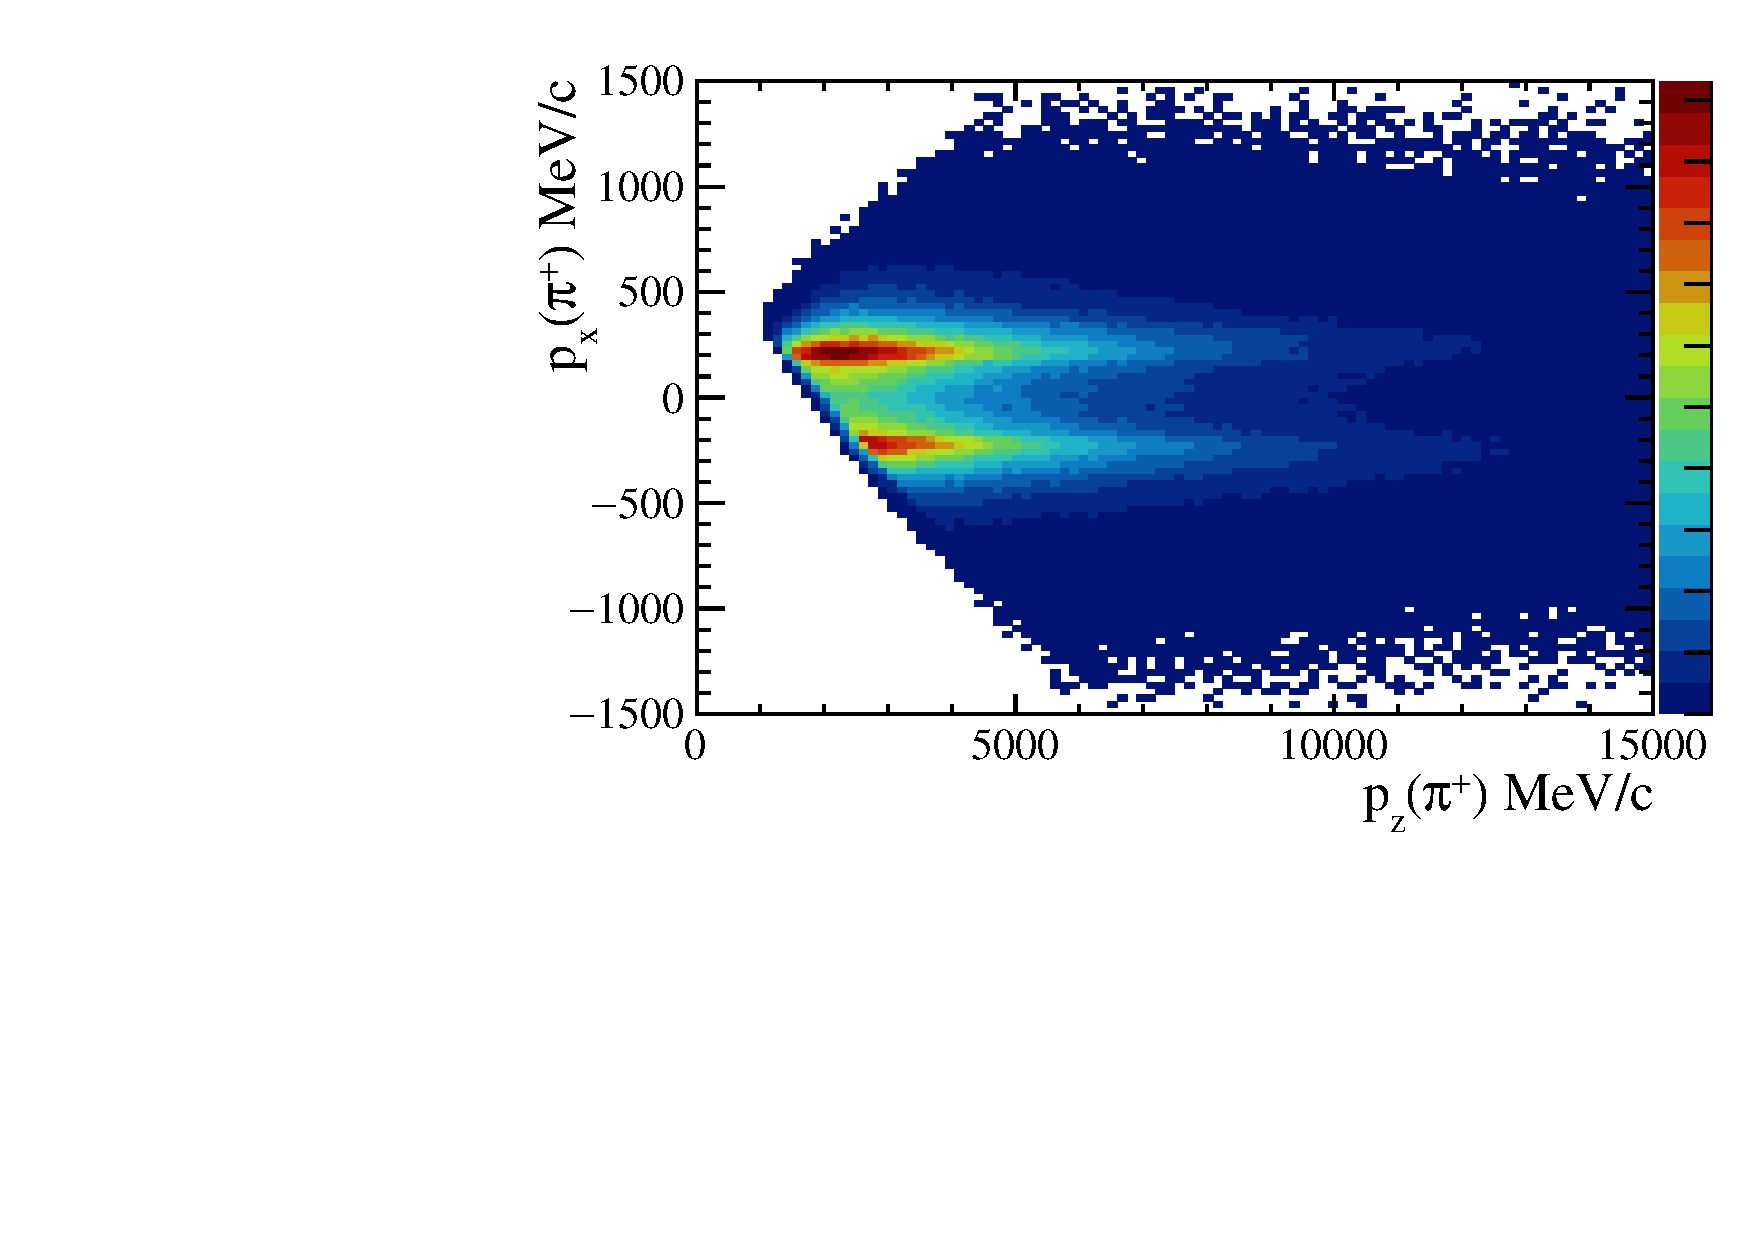
\includegraphics[width = 0.5\textwidth]{../work/RapidSimAnalysis/PGunAnalysis/Plots/KK_Dst_PXPZ_Positive.pdf}}
                \subfloat{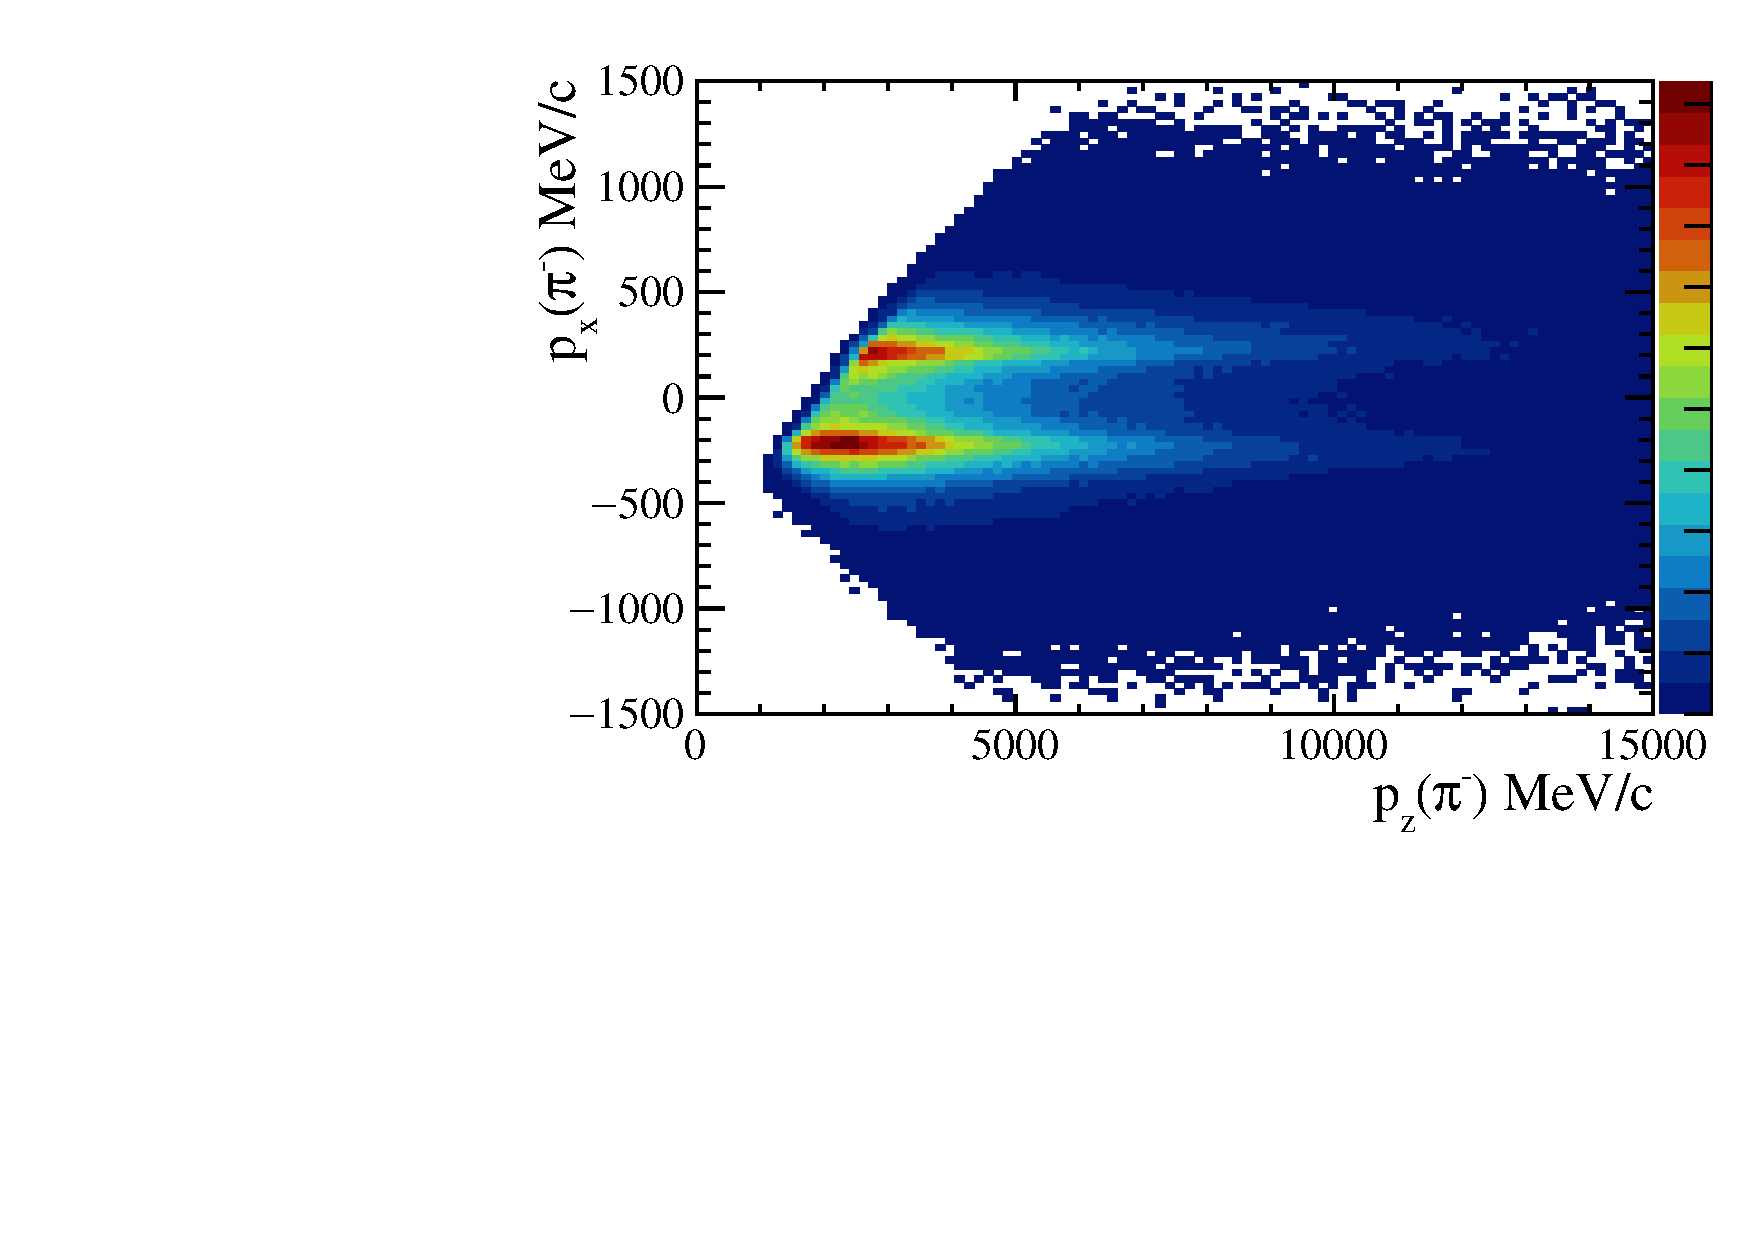
\includegraphics[width = 0.5\textwidth]{../work/RapidSimAnalysis/PGunAnalysis/Plots/KK_Dst_PXPZ_Negative.pdf}}
                \caption{We present the positive (left) and negative (right) soft pion $p_x - p_z$ momentum planes for the $D^0\to K^-K^+$ sample generated using Particle Gun.}
                \label{fig:detection_pgun}
        \end{figure}

        We present the distribution of the weighting function values in Fig.~\ref{fig:weightingPgun}.
        With the implementation of the weighting function, the detection asymmetries should cancel out when calculating $\Delta A_\text{total}$, thus the calculated value should be consistent with zero.

        \begin{figure}[h!]
                \centering
                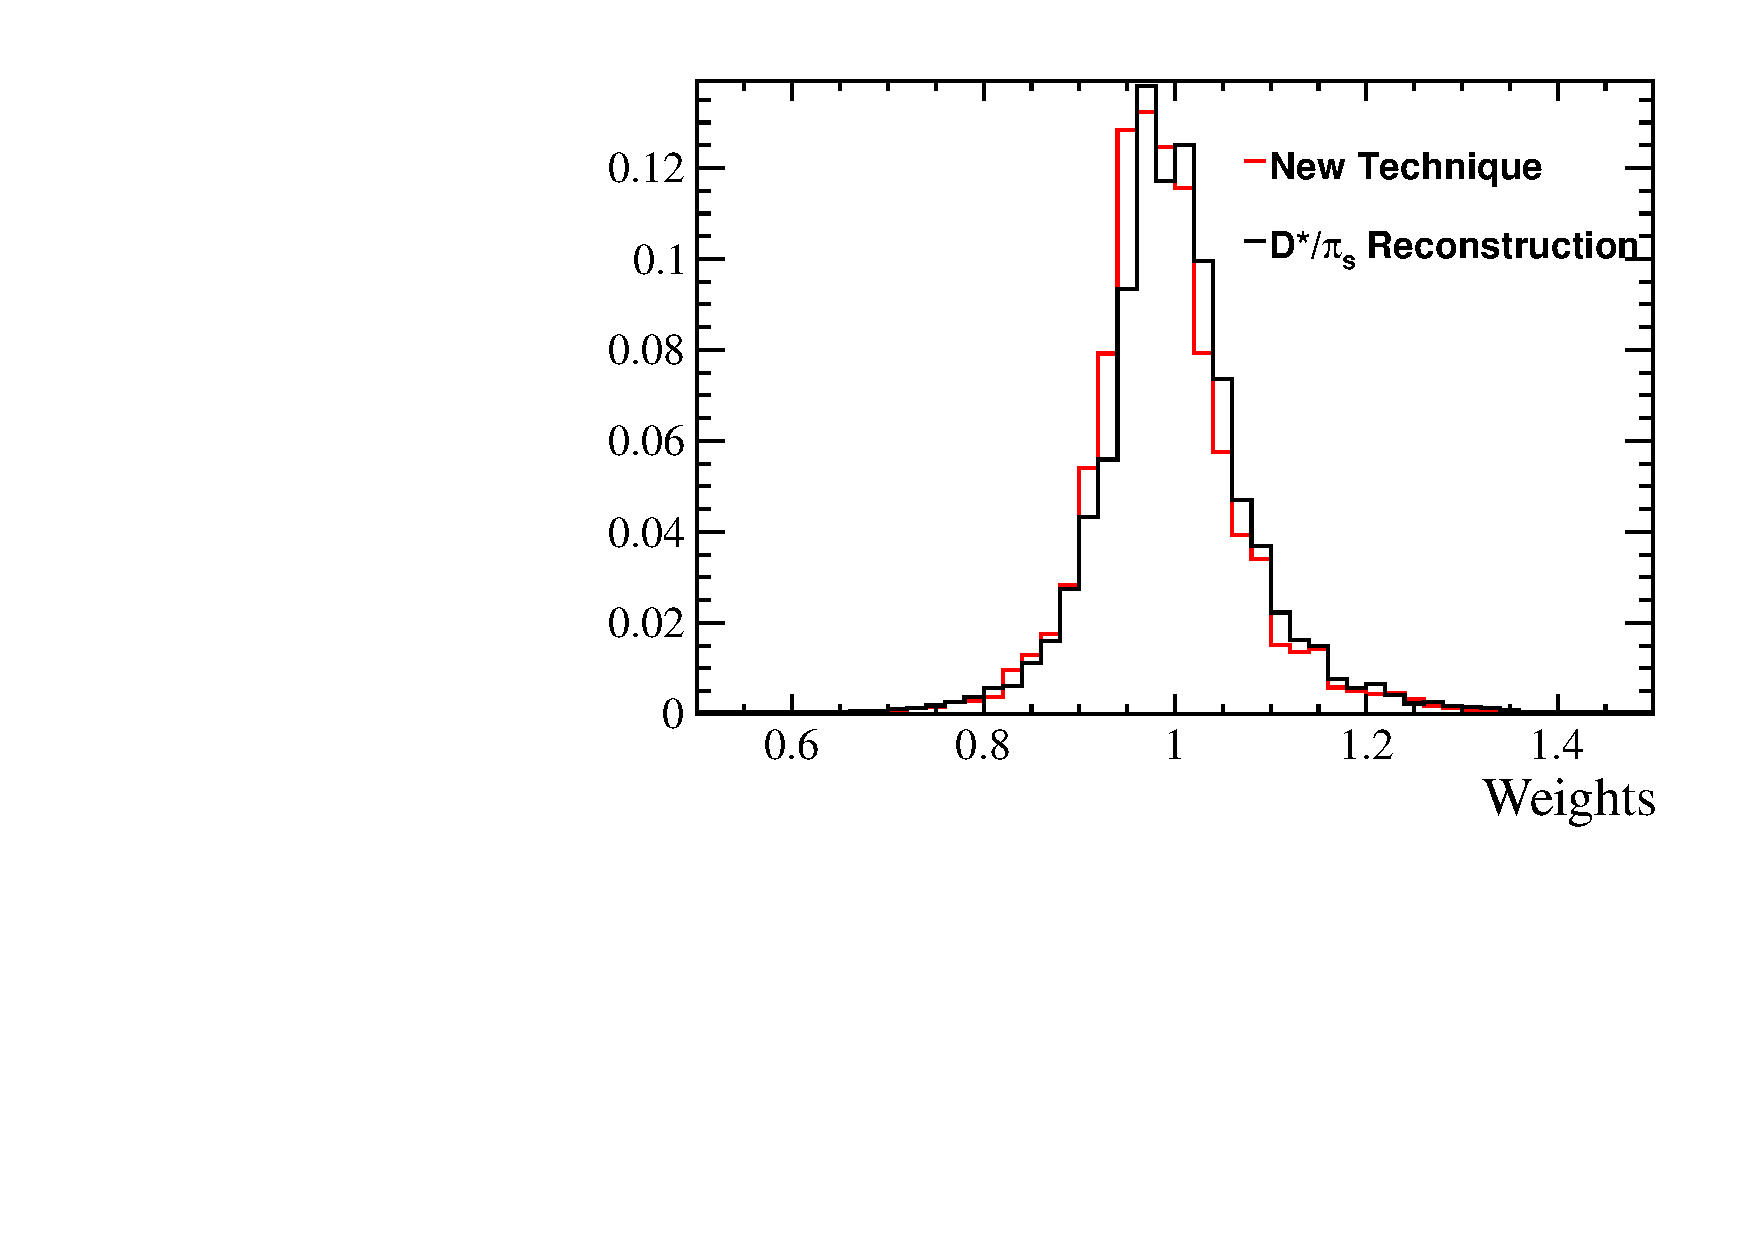
\includegraphics[width = 0.7\textwidth]{../work/RapidSimAnalysis/PGunAnalysis/Plots/Weights.pdf}
                \caption{Normalized weighting function distributions obtained from the $D^0$ and $D^\star$ samples.}
                \label{fig:weightingPgun}
        \end{figure}

        Using the same procedure as before, we calculate the total asymmetries of the two samples and the total asymmetry difference.
        Our results are shown in Tab.~\ref{tab:asymmetries_total_pgun} for the $D^0\to K^-K^+$ sample, while for the $D^0\to\pi^-\pi^+$ sample we get
        \begin{equation}
                A_\text{total} = -0.00024 \pm 0.00074
        \end{equation}
        \begin{center}
                \begin{tabular}{c|c|c}
                        & Weighted & Unweighted\\
                        \hline\hline
                        $D^0$ weighting & $-0.00023 \pm 0.00079$ & \multirow{2}{*}{$0.000016 \pm 0.000787$}\\
                        \cline{1-2}
                        $D^\star$ weighting & $-0.000018 \pm 0.000790$ & \\
                \end{tabular}
                \captionof{table}{We present the $A_\text{total}$ for the $D^0\to K^-K^+$ Particle Gun sample with weights from two different samples and without weights.}
                \label{tab:asymmetries_total_pgun}
        \end{center}

        Using the total asymmetries we calculate the total asymmetry difference between the $D^0\to K^-K^+$ and $D^0\to \pi^-\pi^+$ samples.
        The results are shown in Tab.~\ref{tab:asymmetry_difference_pgun}.

        \begin{center}
                \begin{tabular}{c|c|c|c}
                        & $D^0$ Weighting & $D^\star$ Weighting & Unweighted\\
                        \hline\hline
                        $\Delta A_\text{total}$ & $0.00001 \pm 0.00108$ & $0.00022 \pm 0.00108$ & $0.00026 \pm 0.00108$\\
                        \hline
                        Deviation $(\sigma)$ & 0.009 & 0.20 & 0.24\\
                \end{tabular}
                \captionof{table}{Total asymmetry difference and deviation from the expected value.}
                \label{tab:asymmetry_difference_pgun}
        \end{center}

        Lastly, we present the kinematics of $D^0$ with and without weighting in Fig.~\ref{fig:kimenaticspgun}

        \begin{figure}[h!]
                \centering
                \subfloat{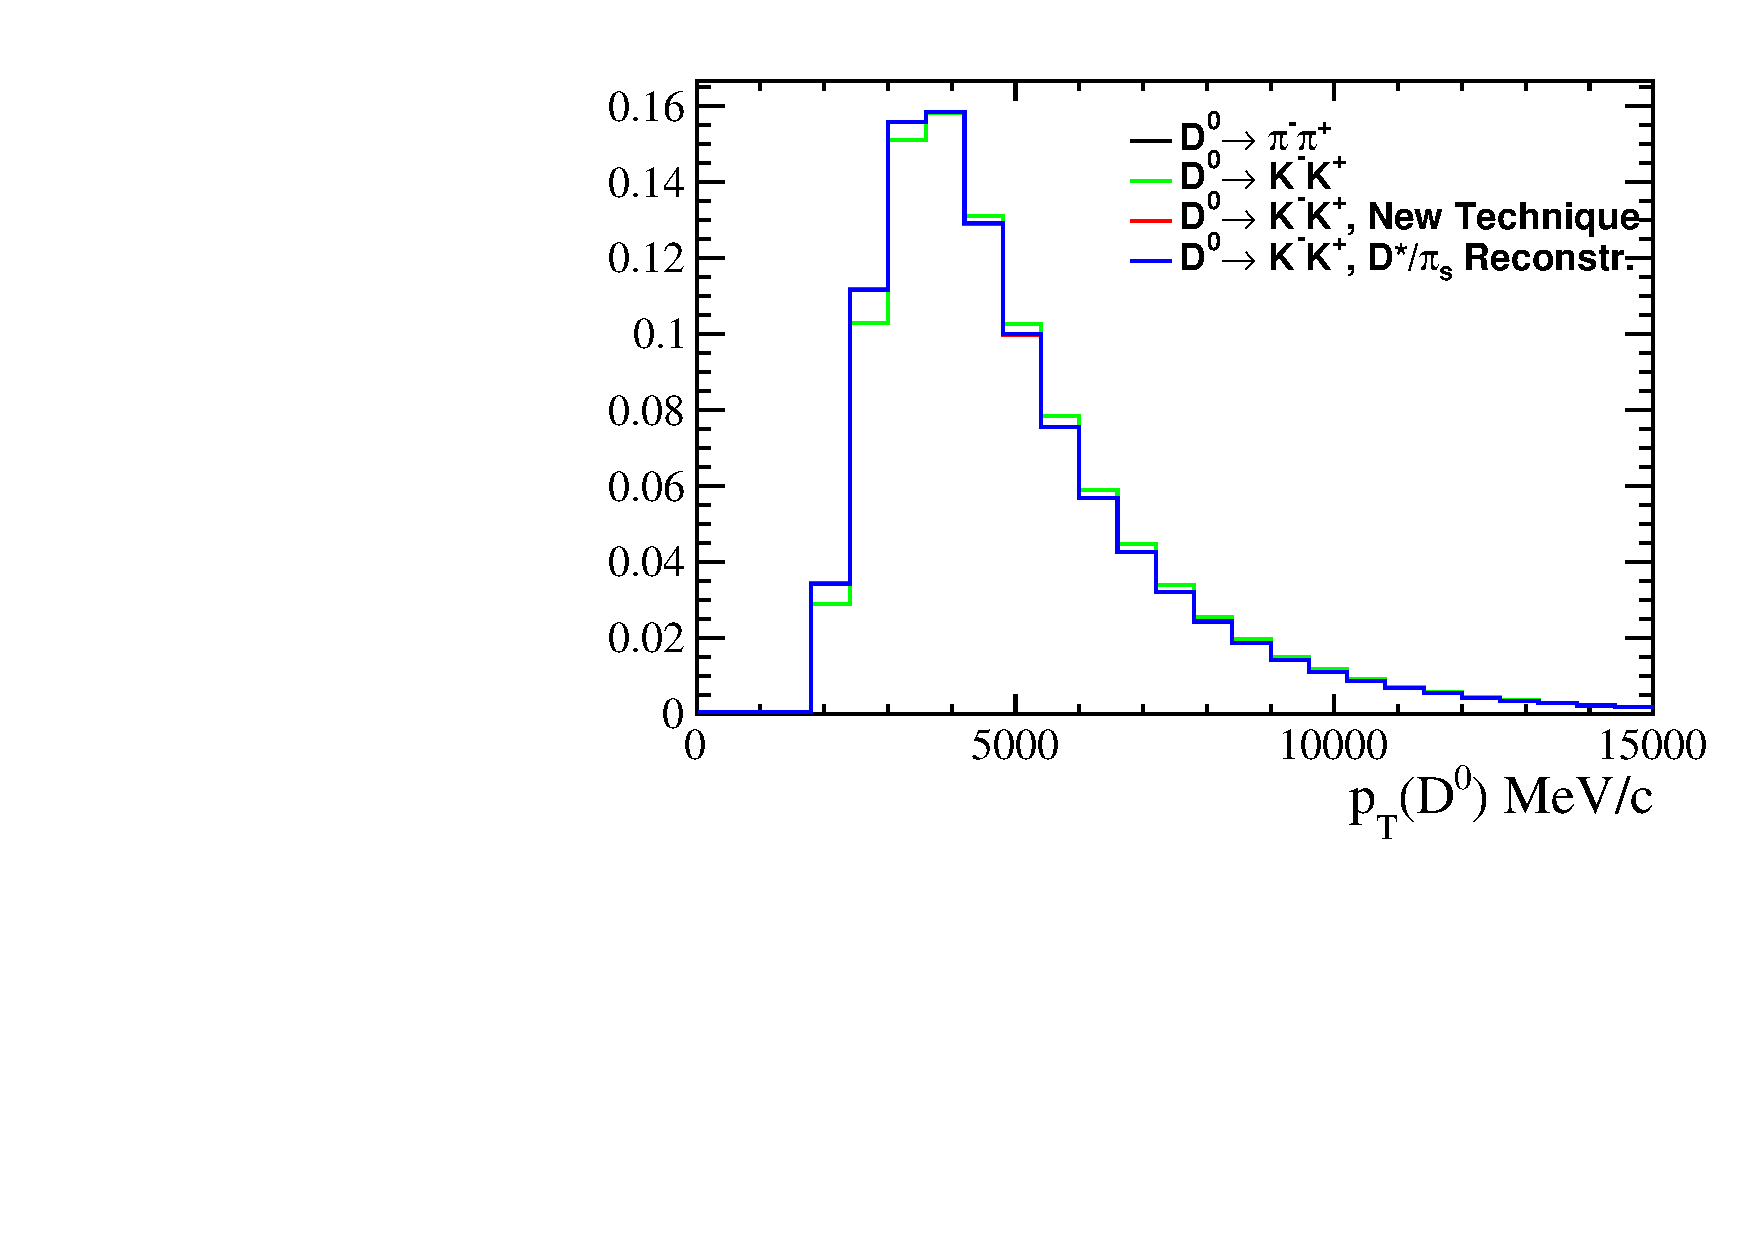
\includegraphics[width = 0.5\textwidth]{../work/RapidSimAnalysis/PGunAnalysis/Plots/D0_PT.pdf}}
                \subfloat{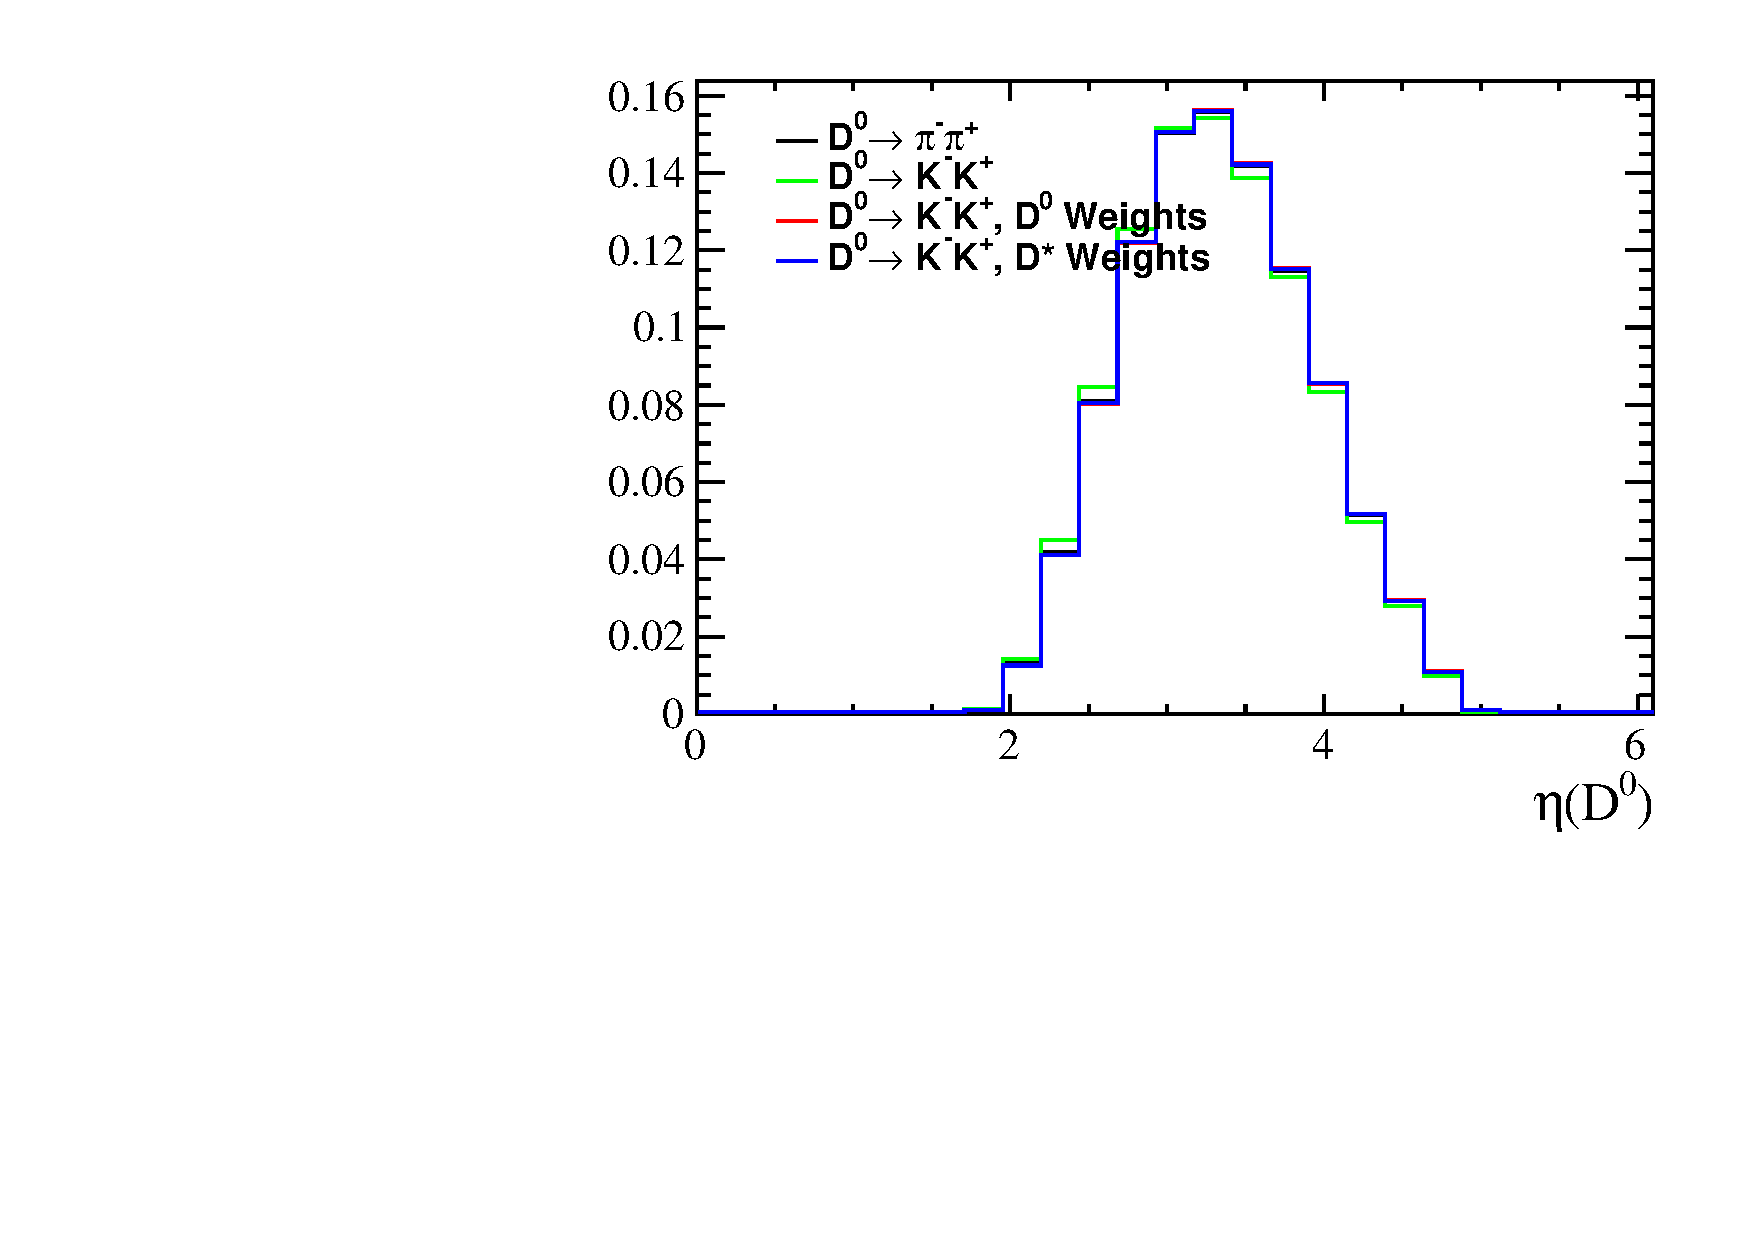
\includegraphics[width = 0.5\textwidth]{../work/RapidSimAnalysis/PGunAnalysis/Plots/D0_ETA.pdf}}
                \hfill
                \subfloat{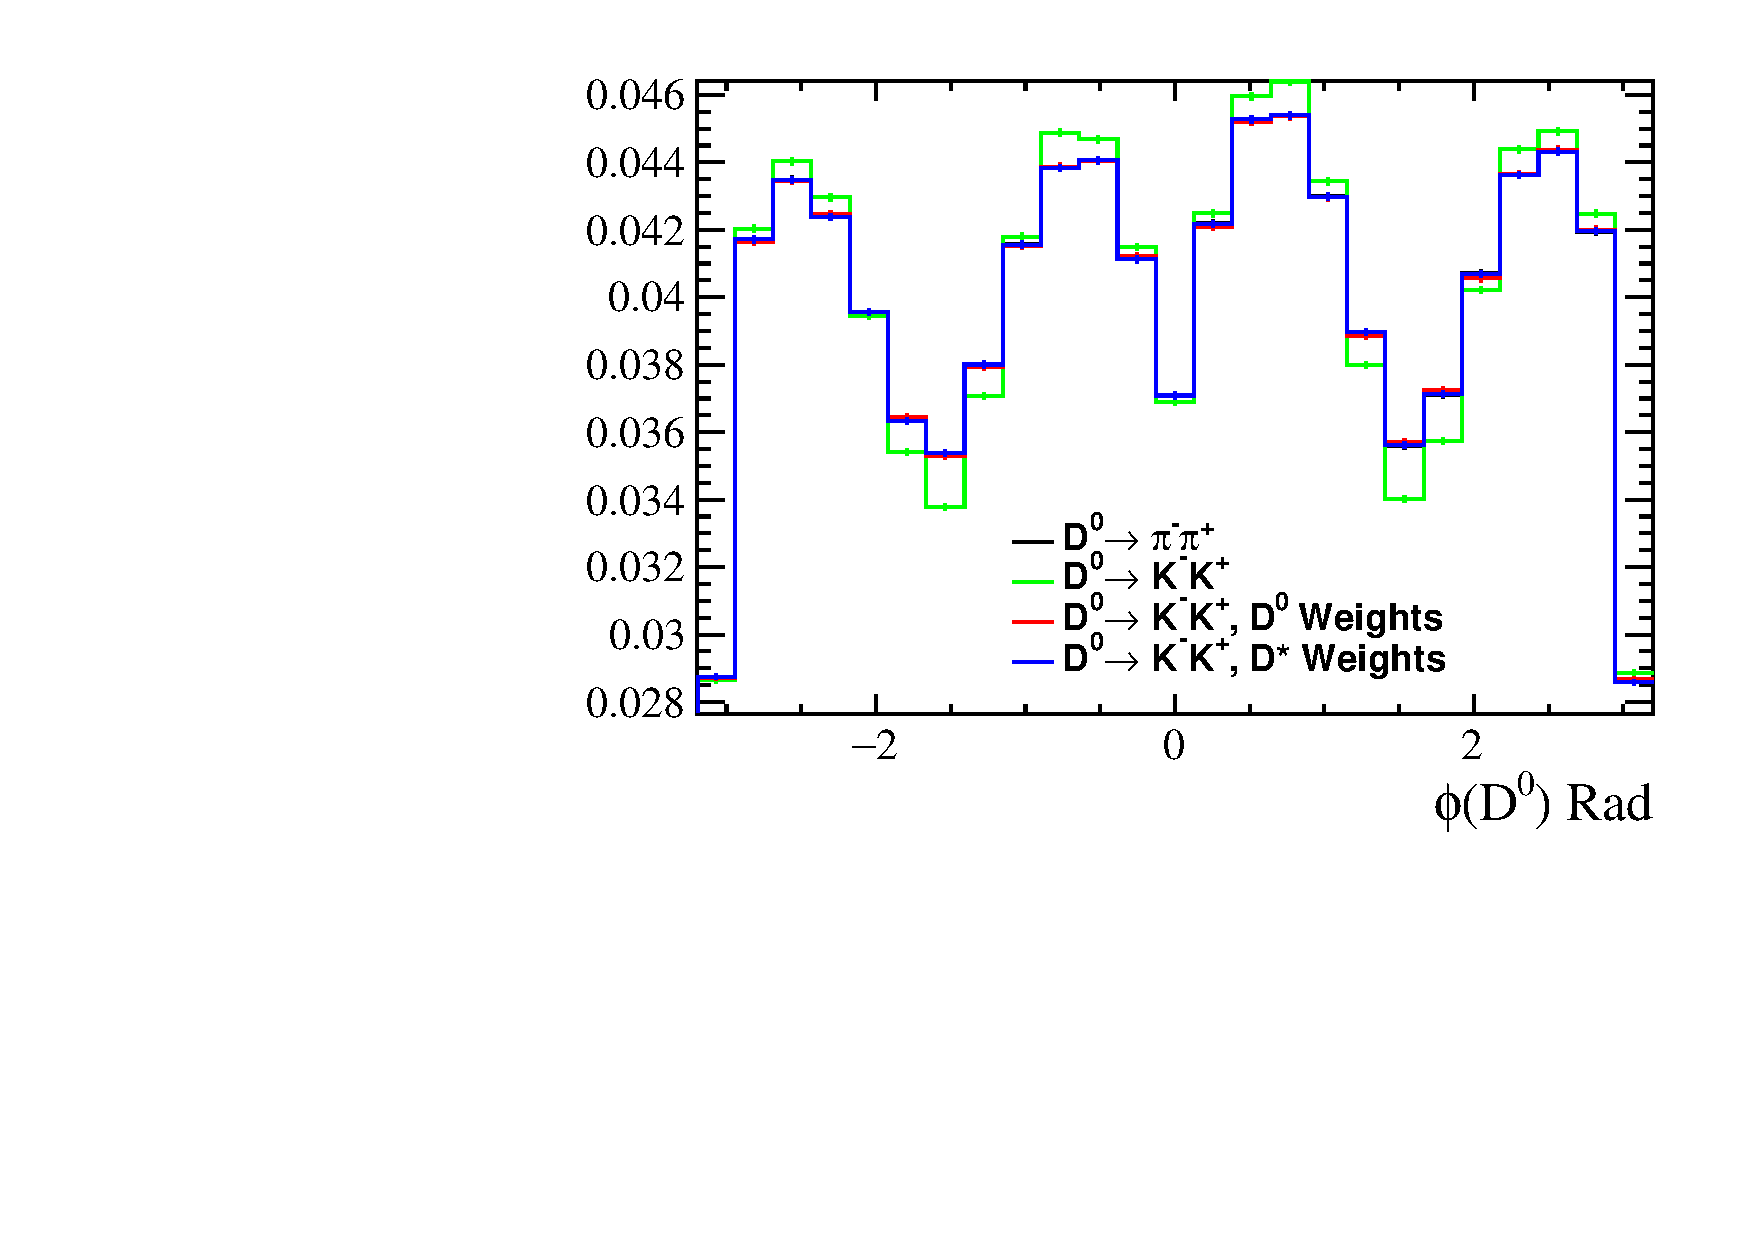
\includegraphics[width = 0.5\textwidth]{../work/RapidSimAnalysis/PGunAnalysis/Plots/D0_PHI.pdf}}

                \caption{We present the $D^0$ normalized kinematic distributions with and without weighting for the two Particle Gun samples.}
                \label{fig:kimenaticspgun}
        \end{figure}

        \section{Conclusions}
        As demonstrated the weighting function allows us to keep events with kinematics associated with large detection asymmetries.
        As demonstrated in the RapidSim data analysis the weighting function slightly reduces the deviation of $\Delta A_\text{total}$ for the case of weighting after the detection asymmetry.
        However, if the calculation of the weighting function predates the introduction of the detection asymmetry, then we observe a significant improvement of our results.

        For the case of Particle Gun data, all measurements are consistent with the expected value of zero, however we notice that the weighting using the $D^0$ samples yields a much smaller deviation.

        Furthermore, we observe from the kinematic distributions of $D^0$ that the weighting function essentially equalizes the kinematics of $D^0\to K^-K^+$ and $D^0\to \pi^-\pi^+$, which is expected, since the weight value is the ratio of the two.
        
        In conclusion, the weighting function we examined can be effectively used in further analyses using LHCb data where detection soft pion detection asymmetries with similarities to our results occur and are otherwise discarded.
        


        \pagebreak
        \nocite{*}
        \printbibliography[notcategory=cited]
        \addcontentsline{toc}{chapter}{Bibliography}
\end{document}